\documentclass{report}

\usepackage{ugentstyle}
\usepackage{caption}
\DeclareCaptionFormat{empty}{} % lege captions

\begin{document}
\maketitle{Computergrafiek - Examen}
\tableofcontents



\chapter{Modelvragen eerste theorievraag}
Deze vraag wordt gequoteerd op 1/4 van de totaalpunten.
\section{Rastering}
\begin{enumerate}
	\vraag
	{
		Bespreek de verschillende algoritmen voor de \textit{rastering van rechte lijnen}, zonder in detail in te gaan op \textit{multi-step} varianten. Vermeld telkens hun voor- en nadelen. \accentuate{(§1.2 \& §1.2.1)}
	}
	{
		\begin{itemize}
			\item \textbf{Midpoint subdivision.} Dit algoritme maakt gebruik van een recursieve procedure waarbij het midden van een lijnstuk berekent wordt, de overeenkomstige pixel selecteert, en daarna deze procedure opnieuw aanroept om de twee helften van het segment. Dit algoritme werkt nadelig naarmate een hellingshoek van 45 graden bereikt wordt. Het effect is dan onregelmatig en dunner. Het grootste nadeel is echter dat het me reële getallen moet uitgevoerd worden.
			      				
			\item \textbf{Asymmetrische DDA.} Algoritmes van de familie DDA pogen het aantal reële getallen te beperken, en voeren hun berekeningen ook incrementeel uit in plaats van recursief. Bij asymmetrische DDA wordt de x-waarde wordt telkens met 1 verhoogt terwijl de y-waarde verhoogt wordt met de richtingscoëfficiënt van de rechte. In elke stap wordt een pixel berekend en geselecteerd. Indien de helling van de rechte met de x-as groter zou zijn dan 45 graden, worden de rollen van x en y omgewisseld. Hier is echter ook het probleem dat indien de hellingshoek 45 graden nadert, dat de lijn te dun wordt getekend.
			      				
			\item \textbf{Symmetrische DDA.} De symmetrische variant van DDA vermijdt het onderscheid in functie van de hellingshoek ten opzichte van de x-as, door de incrementen in beide richtingen repetitief te halveren tot wanneer deze kleiner zijn dan een pixel. Nadat de incrementen berekend zijn, wordt hetzelfde princiepe toegepast als asymmetrische DDA. De x en y-waarde worden nu telkens verhoogt met de eerder berekende incrementen, en selecteren de juiste pixel. Aangezien de incrementen kleiner zijn dan een pixel, zullen sommige pixels meerdere malen geselecteerd worden, wat een impact heeft op de snelheid van het algoritme. Het resultaat indien de hellingshoek 45 graden nadert, is voller dan by de asymmetrische variant, maar het patroon is minder regelmatig. Het produceert hetzelfde resultaat als midpoint subdivision.
			      				
			\item \textbf{Kwadrant DDA.} Dit algoritme verhoogt de incrementen met exact 1 pixel, maar nooit in beide richtingen tegelijkertijd. De verhouding van het aantal incrementen in de y-richting tot het aantal incrementen in de x-richting wordt bepaald door de richtingscoëfficiënt van de rechte. Er is een extra variabele, $\Delta$ die best geinitialiseerd wordt op $\frac{(x_2 - x_1) - (y_2 - y_1)}{2}$. Indien $\Delta$ foutief geinitialiseerd wordt, produceert dit algoritme slechte resultaten bij zeer vlakke of zeer steile lijnstukken. De variabele $\Delta$ bepaalt of de lijn verder getekend moet worden in de x-richting, indien $\Delta \geq 0$, of in de y-richting wanneer $\Delta < 0$.
			      				
			      Een enorm voordeel van dit algoritme is dat het geen gebruik maakt van reële getallen, ook niet bij de  variabele $\Delta$ aangezien het dubbele bijgehouden wordt. Bij een hellingshoek die 45 graden nadert, zijn de lijnstukken veel te dik. Dit is logisch aangezien de helft van de beslissingen het lijnstuk in de x-richting zullen selecteren, en de andere helft in de y-richting, telkens afwisselend van elkaar.
			      				
			\item \textbf{Octant DDA.} Dit laatste algoritme verfijnt kwadrant DDA door overlappende segmenten te vermijden. Indien de hellingshoek van het lijnstuk kleiner zou zijn dan 45 graden, zal octant DDA een pixel ofwel in de horizontale richting of in de diagonale richting selecteren, afhankelijk naargelang $\Delta$ positief of negatief is. Is de hellingshoek groter, dan zal octant DDA in de verticale of diagonale richting selecteren. 
			      				
			      Dit algoritme produceert ongeveer dezelfde resultaten als asymmetrische DDA, zonder gebruik te maken van reële getallen. Naarmate de hellingshoek 45 graden nadert, wordt het lijnstuk te fijn weergegeven.
		\end{itemize}
	}
		
			
	\vraag
	{
		Hoe kunnen de methodes aangepast worden om \textbf{dikke} lijnen voor te stellen? \accentuate{(§1.5)}
	}
	{
		\begin{itemize}
			\item \textbf{Replicatie.} Dit is een eenvoudige manier, dat bij elke iteratie van een DDA algoritme, enkele pixels boven en onder, of links en rechts van de geselecteerde pixels meeselecteren, afhankelijk van de gewenste dikte en de hellingshoek. De overgang tussen twee lijnstukken die op deze manier dikker gemaakt zijn, is niet altijd even goed. Deze techniek wordt enkel toegepast indien de lijnen relatief dun zijn.
			\item \textbf{Replicatie met vorm.} Bij elke iteratie van een DDA algoritme wordt rond de huidige geselecteerde pixel, een vlak geselecteerd. Vaak gebruikte vlakken zijn vierkanten voor lijnstukken en cirkelvormige vlakken voor cirkels.
			      				
			\item \textbf{Opvulling.} Een derde techniek is om tweemaal het DDA algoritme toe te passen, op lijnstukken die uit elkaar verschoven zijn. Daarna worden deze twee lijnstukken opgevuld met de techniek om veelhoeken op te vullen.
		\end{itemize}
	}
			
\end{enumerate}

\section{Het algoritme van Bresenham}
\begin{enumerate}
	\vraag
	{
		Bespreek het doel van dit algoritme en geef de volledige uitwerking van het selectieproces. \accentuate{(§1.3)}
	}
	{
		\begin{itemize}
			\item Het algoritme van Bresenham is geschikt om pixels te rasteren in de vorm van een cirkel terwijl het ook enkel gehele getalllen vereist. Het algoritme berekent enkel de pixels voor de cirkelsector met beginpunt ($0, R$) en eindpunt ($R/\sqrt{2},R/\sqrt{2}$). De andere cirkelsectoren kunnen met behulp van symmetrie bekomen. Bij elke iteratie wordt de x-waarde van de pixel verhoogd. Het aanpassen van de y-waarde hangt af van de discriminant $\Delta_i$. Is deze waarde strikt positief dan zal de y-waarde met 1 pixel verlaagt worden. Is de discriminant negatief, dan blijf de y-waarde dezelfde. De discriminant $\Delta_i$ wordt gedefinieerd als het verschil van de kwadraten van de afstanden van de twee mogelijke punten tot de cirkel:
			      				
			      \begin{equation*}
			      	\begin{split}
			      		\Delta_i & = [(x_{i - 1} + 1)^2 + y_{i - 1}^2 - R^2] - [R^2 - (x_{i - 1} + 1)^2 - (y_{i - 1} - 1)^2]  \\
			      		& = 2(x_{i - 1} + 1)^2 + y_{i - 1}^2 + (y_{i - 1} - 1)^2 - 2R^2
			      	\end{split}
			      \end{equation*}	
			      				
			      De discriminant $\Delta_{i + 1}$ kan uit $\Delta_i$ afgeleidt worden.
			      \begin{equation*}
			      	\begin{split}
			      		\Delta_{i + 1} & = 2(x_{i - 1} + 2)^2 + y_i^2 + (y_i - 1)^2 - 2R^2 \\
			      		& = \Delta_i + 4x_i + 6 + y_i^2 - y_{i - 1}^2 + (y_i - 1)^2 - (y_{i - 1} - 1)^2 \\
			      		& = \begin{cases}
			      		\Delta_i + 4x_{i - 1} + 6 &, \Delta_i \leq 0 \\
			      		\Delta_i + 4(x_{i - 1} - y_{i - 1}) + 10  &, \Delta_i > 0
			      		\end{cases}
			      	\end{split}
			      \end{equation*}
			      				
			      De beginwaarde van de discriminant, $\Delta_i$ kan bekomen worden door de substitutie $x_{i - 1} = 0$ en $y_{i - 1} = R$ toe te passen:
			      $$\Delta_1 = 3 - 2R$$
			      				
		\end{itemize}
		
	}
	
			
	\vraag
	{
		Hoe kunnen de methodes aangepast worden om \textbf{dikke} lijnen voor te stellen? \accentuate{(§1.5)}
	}
	{
		\begin{itemize}
			\item \textbf{Replicatie.} Dit is een eenvoudige manier, dat bij elke iteratie van een DDA algoritme, enkele pixels boven en onder, of links en rechts van de geselecteerde pixels meeselecteren, afhankelijk van de gewenste dikte en de hellingshoek. De overgang tussen twee lijnstukken die op deze manier dikker gemaakt zijn, is niet altijd even goed. Deze techniek wordt enkel toegepast indien de lijnen relatief dun zijn.
			\item \textbf{Replicatie met vorm.} Bij elke iteratie van een DDA algoritme wordt rond de huidige geselecteerde pixel, een vlak geselecteerd. Vaak gebruikte vlakken zijn vierkanten voor lijnstukken en cirkelvormige vlakken voor cirkels.
			      				
			\item \textbf{Opvulling.} Een derde techniek is om tweemaal het DDA algoritme toe te passen, op lijnstukken die uit elkaar verschoven zijn. Daarna worden deze twee lijnstukken opgevuld met de techniek om veelhoeken op te vullen.
		\end{itemize}
	}
\end{enumerate}

\section{Rastering van veelhoeken en antialiasing}
\begin{enumerate}
	\vraag{
		Hoe moeten algoritmen voor het rasteren van rechte lijnen gewijzigd worden indien men ze wil toepassen op het \textit{opvullen van veelhoeken}? \accentuate{(§1.4)}
	}
	{
		\begin{itemize}
			\item De veelhoek wordt afgetast met een horizontale of verticale scanlijnen. Voor elke scanlijn worden de intersectiepunten met de lijn en het veelhoek bepaalt. Het aantal intersectiepunten is altijd een even aantal. De intersecties worden (bij een horizontale scanlijn) gesorteerd op de x-waarde. Alle pixels x tussen een intersectie met een even index en een intersectie met oneven index, $x_{2i} \leq x \leq x_{2i + 1}$ , worden getekend. Om te voorkomen dat pixels buiten het veelvlak geselecteerd worden, beperkt men de selectie tot enkel inwendige pixels als intersectiepunten, ook als ligt een uitwendig pixel dichter bij de randlijn. 
		\end{itemize}
	}
			
	\vraag
	{
		Geef het doel van \textit{antialiasing}, het algemeen principe ervan, en drie algoritmen voor de praktische uitwerking (met voorbeelden). \accentuate{(§1.6)}
	}
	{
		\begin{itemize}
			\item Antialiasing is het proces om de discrete eigenschap dat pixels vertonen, namelijk het gekarteld uitzicht, te minimaliseren. 
			      \begin{enumerate}
			      	\item \textbf{Supersampling.} Deze techniek maakt gebruik van een interne geheugenbuffer. Deze buffer biedt een fijner raster aan dan die dat hardwarematig beschikbaar zijn. Een pixel op een computerscherm kan overeenkomen met 16 pixels in het geheugen. Na het rasteringsproces, dat nu uitgevoerd wordt in het geheugen, wordt voor elke pixel nagegaan hoeveel geheugenpixels in de groep geselecteerd zijn. Als 7 pixels geselecteerd zijn met een geheugenpixelgrootte van 16 pixels, dan zal die pixel een intensiteit van $7/16$ bedragen.
			      	\item \textbf{Postfiltering.} Deze methode zal eerst het rasteringsproces uitvoeren in het geheugen, dat nu dezelfde resolutie heeft als de hardware. Nadien wordt de intensiteit van een pixel herberekend op basis van het al dan niet geselecteerd zijn van de naburige pixels. De groep dat in beschouwing wordt genomen heeft vaak de vorm van een rechthoek (meer specifiek, een vierkant). Het gewicht van een naburige pixel wordt berekend op basis van de afstand van die pixel tot het middenpunt van de groep.
			      	\item \textbf{Prefiltering.} In tegenstelling tot de vorige twee algoritmen zal het rasterproces en antialiasingproces zich in dezelfde stap plaatsvinden. Dit algoritme heeft nood aan aangepaste DDA algoritmen. Een specifieke implementatie is het Pitteway-Watkinson algoritme. Dit algoritme maakt het mogelijk om een pixel te selecteren terwijl zijn intensiteit incrementeel berekend wordt. \todo{??}
			      \end{enumerate}
		\end{itemize}
	}
\end{enumerate}

\section{Transformaties}
\begin{enumerate}
	\vraag
	{
		Welke families transformaties worden in de computer-grafiek gebruikt, en waarom?
	}
	{
		\begin{itemize}
			\item \textbf{Affiene transformaties.} Hieronder vallen de rotaties, schaaloperaties, spiegelingen en translaties. Deze transformaties behouden colliniariteit en parallellisme. Evenwijdige lijnen zullen na een affiene transformatie nog steeds evenwijdig zijn. 
			      			
			\item \textbf{Perspectieve projecties.} Deze transformaties maken het mogelijk om een driedimensionaal object voor te stellen op een tweedimensionaal uitvoerapparaat.
			      			
			\item De combinatie van deze twee transformaties biedt de mogelijkheidt om onder andere:
			      \begin{itemize}
			      	\item een object vanuit een andere kijkrichting te bekijken.
			      	\item hij construeren van een object dat uit meerdere identieke componenten bestaat. 
			      \end{itemize}
		\end{itemize}	
	}
		
	\vraag 
	{
		Geef en bespreek de matrixrepresentaties van de verschillende types transformaties en hun samenstellingen. \accentuate{(§2.1 behalve §2.1.4)}	
	}
	{
		\begin{itemize}
			\item \textbf{Rotaties.} 
		\end{itemize}
	}
\end{enumerate}

\section{Projecties en clipping}

\begin{enumerate}
	\vraag{Welke soort projectie wordt in de computergrafiek gebruikt, en waarom?}{ 	
		\begin{itemize}
			\item De computergrafiek maakt gebruik van perspectieve projecties. Deze soort projecties simuleren de werking van het menselijk oog. Er wordt een oogpunt en een kijkrichting vastgelegd. De kijkrichting is een georiënteerde rechte door het oogpunt. Tussen het oogpunt en elk object wordt een rechte verbonden. Ergens op die rechte zal er een snijpunt zijn met het projectievlak. Dit snijpunt bepaalt het getransformeerde beeld van het punt.
		\end{itemize} 
	}
		
	\vraag{Leid de algemene matrixvorm van deze projectie af. \accentuate{(§2.2)}}{
		\begin{itemize} 
			\item Een perspectieve projectie kan afgeleid worden na het toepassen van een affiene transformatie. Een translatie T verplaatst het snijpunt van de kijkrichting met het projectievlak naar de oorsprong van het coördinatenstelsel. Deze transformatie wordt gevolgd door een rotatie R die het oogpunt op de negatieve z-as plaatst, in het punt met homogene coördinaten (0, 0, -d, 1). Hierdoor valt het projectievlak samen met het xy-vlak. Hierdoor is ook de z-waarde van het geprojecteerd punt nul. Op dit moment kunnen twee driehoeken beschouwd worden. De driehoek met de kijkrichting vanuit de y-as naar het zx-vlak (1) en de driehoek met de kijkrichting vanuit de x-as naar het zy vlak (2).
			      \begin{enumerate}
			      	\item[(1)] Hieruit kan afgeleidt worden dat $\frac{x_p}{d} = \frac{d}{z + d}$.
			      	\item[(2)] Hieruit kan afgeleidt worden dat $\frac{y_p}{d} = \frac{d}{z + d}$.
			      \end{enumerate}
			      In homogene coördinaten kan dit echter vereenvoudigd worden.:
			      $$x' \equiv w'\cdot x_p = x \qquad y' \equiv w'\cdot y_p = y \qquad \hbox{met} \qquad w' = \frac{z}{d} + 1$$
			      In matrixvorm:
			      $$
			      \begin{pmatrix}
			      	x' \\ y' \\ 0 \\ w'
			      \end{pmatrix}
			      =
			      \begin{pmatrix}
			      	1 & 0 & 0   & 0 \\
			      	0 & 1 & 0   & 0 \\
			      	0 & 0 & 0   & 0 \\
			      	0 & 0 & 1/d & 1 \\
			      \end{pmatrix} 
			      \cdot
			      \begin{pmatrix}
			      	x \\ y \\ z \\ 1
			      \end{pmatrix}
			      $$
			      		
			      Hieruit is het duidelijk dat een perspectieve projectie ook kan berekend worden via eenvoudige matrixvermenigvuldigingen:
			      $$
			      \begin{pmatrix}
			      	x' \\ y' \\ 0 \\ w'
			      \end{pmatrix}
			      =
			      \begin{pmatrix}
			      	1 & 0 & 0   & 0 \\
			      	0 & 1 & 0   & 0 \\
			      	0 & 0 & 0   & 0 \\
			      	0 & 0 & 1/d & 1 \\
			      \end{pmatrix} 
			      \cdot
			      \begin{pmatrix}
			      	i_x & j_x & k_x & -\theta_x \\
			      	i_y & j_y & k_y & -\theta_y \\
			      	i_z & j_z & k_z & -\theta_z \\
			      	0   & 0   & 0   & 1         
			      \end{pmatrix}
			      \cdot
			      \begin{pmatrix}
			      	x \\ y \\ z \\ 1
			      \end{pmatrix}
			      $$
		\end{itemize}
	}
		
	\vraag{Wat is de bedoeling van clipping? Bespreek clippen in twee en in drie dimensies. \accentuate{(§2.3 zonder deelparagrafen)}}{
		\begin{itemize} 
			\item Een kijkrichting is begrensd door een bepaalde maximumwaarde. Vanuit het oogpunt kan er een pyramide beschouwd worden. Elke pixel dat zich niet in deze pyramide bevindt moet geclipt worden, aangezien deze toch niet gezien kan worden. De doorsnede van de pyramide met het projectievlak wordt het viewport genoemd. De viewport is evenwijdig met de x- en y-assen met het centrum in de oorsprong van het coördinatenstelsel waarin het geprojecteerd beeld afgebeeld. De selectie van alle pixels in perspectieve projectie die binnen de viewport liggen noemt men clipping. 3D Objecten worden eerste geclipt vooraleer ze perspectief geprojecteerd wordt. 2D objecten worden geprojecteerd en daarna pas geclipt. Het clippen van lijnstukken en opgevulde veelhoeken wordt door vrijwel alle algoritmen ondersteund. Bij het clippen van complexere veelhoeken wordt eerst de omhullende veelhoek berekent, en worden alle zijden geclipt met de viewport.
		\end{itemize}}
\end{enumerate}

\section{Het algoritme van Cyrus-Beck}
\begin{enumerate}
	\vraag{Geef het doel, de toepasbaarheid, en de beperkingen van het algoritme, en de volledige uitwerking van het principe. Pas het algoritme stap-voor-stap toe op volgende viewport \textit{(figuur wordt gegeven)} en een lijnstuk met eindpunten ... .  \accentuate{(§2.3.2)}}{
		\begin{itemize} 
			\item Het algoritme van Cyrus-Beck is geschikt om lijnen te clippen ten opzichte van een willekeurige convexe veelhoek. Het algoritme maakt gebruik van de geparameteriseerde voorstelling van een lijnstuk: $P(t) = P_1 + t(P_2 - P_1)$. Indien $0 \leq t \leq 1$, dan bevindt P(t) zich op het lijnstuk. Het Cyrus-Beck algoritme spoort deze t-waarden op van de intersecties met de verschillende zijden van de viewport en hieruit afleiden ofdat het lijnsegment hetzij partieel, hetzij totaal binnen de viewport ligt.
			      				
			      De eerste stap van dit algoritme berekent alle $n_i[P(t) - f_i]$ functies en de waarden van $t_i$ waarvoor deze functies nul worden. Indien al deze functies niet-negatieve waarden hebben voor zowel $t = 0$ als $t = 1$, dan ligt het lijnstuk volledig binnen de viewport. Is dit slechts het geval voor $t = 0$ of $t = 1$, dan ligt het lijnstuk zeker partieel in de viewport. Er moet bijgevolg extra kandidaatsnijpunten met de viewport gezocht worden. Enkel $t_j$ waarden waarvor $0 \leq t_j \leq 1$ komen hiervoor in aanmerking. Voor elke $t_j$ waarde wordt nagegaan of $n_i \cdot [P(t_j) - f_i] \geq 0$. De kleinste en grootste $t_j$ leveren de gezochte snijpunten op.
			      				
			\item Toegepast op een lijnstuk met punten $P_1(-1, 1)$ en $P_2(9, 3)$ in een viewport met dimensie 8 bij 4 (fig 2.23 p 27 in de cursus). Het lijnstuk wordt geparameteriseerd door $$P(t) = \begin{cases}
			      x = -1 + 10t \\
			      y = 1 + 2t
			\end{cases}$$
			Neem $f_{L, B} = (0, 0)$ en $f_{T, R} = (8, 4)$. Uitrekenen van de $n_i[P(t) - f_i]$ functies wordt dan:
			\begin{table}[h]
				\centering
				\begin{tabular}{c | c | c}
					zijde               & $[P_1P_2]$                                           & nulwaarde \\ 
					\hline 
					\\
					$n_L, f_L = (0, 0)$ & $(-1 + 10t - 0, 1 + 2t - 0) \cdot (1, 0) = -1 + 10t$ & $1/10$    \\
					$n_R, f_R = (8, 4)$ & $(-1 + 10t - 8, 1 + 2t - 4) \cdot (-1, 0) = 9 - 10t$ & $9/10$    \\
					$n_B, f_B = (0, 0)$ & $(-1 + 10t - 0, 1 + 2t - 0) \cdot (0, 1) =  1 + 2t$  & $-1/2$    \\
					$n_T, f_T = (8, 4)$ & $(-1 + 10t - 8, 1 + 2t - 4) \cdot (0, -1) = 3 - 2t$  & $3/2$     \\
				\end{tabular}
			\end{table}
			Elke nulwaarde kan een waarde voor t zijn. 	Er moet echter gelden dat $n_i[P(t_j) - f_i] \geq 0, \forall i$. Dit komt neer op het substitueren van de nulwaarden $t_i$ in elke andere functie en nagaan of dat het resultaat positief is voor elk van deze functies. In dit geval is dit enkel voor $t = 1/10$ en $t = 9/10$. Dit zijn dan ook de punten die snijden met de viewport.
		\end{itemize}
	}
			
	\vraag{Hoe clipt men meer ingewikkelde krommen en figuren?}{\begin{itemize} \item \todo{oplossen} \end{itemize}}
\end{enumerate}

\section{Clipping}
\begin{enumerate}
	\vraag{Het algoritme van \textit{Cohen-Sutherland}: geef het doel, de toepasbaarheid, en de beperkingen van het algoritme, en de volledige uitwerking van het principe. Pas het algoritme toe op relevante voorbeelden. Geef eveneens een variant van de techniek. \accentuate{(§2.3.1)}}{
		\begin{itemize} 
			\item Het algoritme van Cohen-Sutherland is geschikt voor het clippen van lijnstukken ten opzichte van een rechthoekig viewport. Dit algoritme is enkel aan te raden om 2D clipping toe te passen. Het algoritme wenst zo snel mogelijk te detecteren of lijnstukken volledig binnen of buiten het viewport liggen. Het algortime zal aan elk eindpunt van een lijnstuk een bitcode $ b_3b_2b_1b_0$ toekennen. Bit $b_0$ wordt op 1 gezet indien het punt zich links van de viewport bevindt, en een bit $b_1$ identificeert een punt aan de rechterzijde van de viewport. Op dezelfde manier hebben punten onder en boven de viewport respectievelijk bits $b_2 = 1$ en $b_3 = 1$. Een lijnstuk dat volledig binnen de viewport ligt heeft dus twee eindpunten met bitcode $0000$. De twee eindpunten van een lijnstuk AND'en kan twee gevallen opleveren:
			      \begin{enumerate}
			      	\item Indien het resultaat verschillend van $0000$ is, dan ligt het lijnstuk met zekerheid buiten de viewport.
			      	\item Is het resultaat echter $0000$ (zonder dat de bitcodes van beide eindpunten $0000$ is) dan ligt slechts een deel van het lijnstuk in de viewport.
			      \end{enumerate}
			      In dit tweede geval wordt het midden van dit lijnstuk genomen, en wordt het algoritme recursief toegepast op beide helften. Deze iteraties moeten doorgevoerd worden tot wanneer de precisie van een pixel bereikt is. Het voordeel van deze methodiek is dat het performant in de hardware kan uitgevoerd worden. Er is enkel een deling door twee vereist en kan parallel uitgevoerd worden.
		\end{itemize}
	}
			
	\vraag{Het algoritme van \textit{Sutherland-Hodgman}: geef het doel, de toepasbaarheid, en de beperkingen van het algoritme, en de volledige uitwerking van het principe. Pas het algoritme stap-voor-stap toe op volgend voorbeeld: (figuur wordt gegeven) . \accentuate{(§2.3.3)}}{\begin{itemize} \item \todo{oplossen} \end{itemize}}
\end{enumerate}

\chapter{Modelvragen tweede theorievraag}
Deze vraag wordt gequoteerd op 1/4 van de totaalpunten.
	
\section{NURBS constructie van cirkels \accentuate{(\textsection 3.4.8, slides en lesnota's)}}
\begin{enumerate}
	\vraag{Met welke \textit{open-uniforme NURBS} van orde drie (graad twee) kun je een \textit{halve cirkel} (met centrum in de oorsprong en straal 1) tekenen , zonder (reële) knooppunten met meervoudige multipliciteit te moeten gebruiken? Geef de preciese locatie van de \textit{controlepunten} (op een figuur), hun gewichten, en de corresponderende \textit{knopenvector}. Uit hoeveel segmenten bestaat deze NURBS?}
	{\begin{itemize} 
		\item Maak gebruik van de gewichten $\{2, 1, 1, 2\}$ en knopenvector $\{0,0;0,1,2;2;2\}$. Deze NURBS bestaat uit twee segmenten.
		\begin{figure}[ht]
			\centering
			\begin{tikzpicture}[scale=5]
				\node (00) at (1, 0) {00};
				\node (01) at (1,1) {01};
				\node (12) at (-1, 1) {12};
				\node (22) at (-1, 0) {22};
				
				\begin{scope}
					\clip (-1,0) rectangle (1, 1);
					\draw[red] (0, 0) circle (1cm);
				\end{scope}
				
				\draw[green] (00) -- (01);
				\draw[green] (01) -- (12);
				\draw[green] (12) -- (22);
			\end{tikzpicture}
		\end{figure}
		\end{itemize}
	}
			
	\vraag{Toon aan dat deze constructie inderdaad exact een halve cirkel oplevert.}{\begin{itemize} \item \todo{oplossen} \end{itemize}}
			
	\vraag{Construeer van deze NURBS de \textit{uniforme} representatie. Vermeld de conversiestappen om tot dit resultaat te bekomen. Waarom is de constructie van de uniforme representatie belangrijk?}
	{
		\begin{itemize} 	
			\item Elk punt $P_{00} = (1, 0, 1), P_{01} = (1, 1, 1), P_{12} = (-1, 1, 1)$ en $P_{22} = (-1, 0, 1)$ heeft een homogeen coördinaat met $w$ het gewicht van die knoop. Deze punten zijn dus equivalent met $P_{00} = (2, 0, 2), P_{01} = (1, 1, 1), P_{12} = (-1, 1, 1)$ e $P_{22} = (-2, 0 , 2)$. Verder kunnen we uit de open-uniforme knopenvector de uniforme knopenvector afleiden, aangezien die steeds oplopende getallen moet bevatten en de reëele knopen hetzelfde blijven: $\{-2, -1; 0, 1, 2; 3, 4\}$. Aangezien het reëele deel hetzelfde blijft, verandert er aan de punten $P_{01}$ en $P_{12}$ niets. De punten $P_{00}$ en $P_{22}$ bestaan niet meer in de uniforme representatie, en worden vervangen door respectievelijk $P_{-10}$ en $P_{23}$. Via het piramidaal schema krijgen we:
			\begin{figure}[ht]
				\centering
				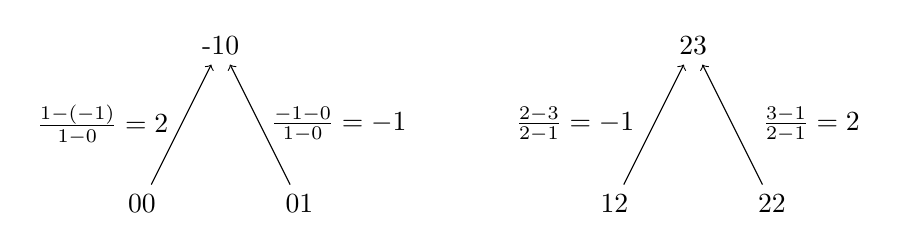
\begin{tikzpicture}
					\node (00) at (0, -1) {00};
					\node (-10) at (1, 1) {-10};
					\node (01) at (2, -1) {01};

					\draw[->] (00) -- node[xshift=-1cm]{$\frac{1 - (-1)}{1 - 0} = 2$}  (-10);
					\draw[->] (01) -- node[xshift=1cm]{$\frac{-1 - 0}{1 - 0} = -1$}  (-10);

					\node (12) at (6, -1) {12};
					\node (23) at (7, 1) {23};
					\node (22) at (8, -1) {22};

					\draw[->] (12) -- node[xshift=-1cm]{$\frac{2 - 3}{2 - 1} = -1$} (23);
					\draw[->] (22) -- node[xshift=1cm]{$\frac{3 - 1}{2 - 1} = 2$}(23);
				\end{tikzpicture}
			\end{figure}

			zodat $$P_{-10} = 2P_{00} - P_{01} = 2 * (2, 0, 2) - (1, 1, 1) = (3, -1, 3)$$ en $$P_{23} = -P_{12} + 2P_{22} = -(-1, 1, 1) + 2 * (-2, 0, 2) = (1, -1, -1) + (-4, 0, 4) = (-3, -1, 3)$$ Uiteindelijk kan men de coördinaten bekomen door elk coördinaat terug om te zetten naar hun twee-dimensionale representatie, zodat $P_{-10} = (1, -\frac{1}{3}), P_{01} = (1, 1), P_{12} = (-1, 1)$ en $P_{23} = (-1, -\frac{1}{3})$ de nieuwe controlepunten worden.

			\item De constructie is belangrijk omdat, indien deze transformatie niet toegepast wordt, het algoritme van Lane en Riesenfeld niet kan toegepast worden. Dit algoritme is namelijk in staat om zeer efficiënt en eenvoudig knopen toe te voegen aan de B-spline, zonder dat de vorm van de B-spline wijzigt. 
		\end{itemize}
	}
\end{enumerate}

\section{NURBS constructie van cirkels en lijnsegmenten \accentuate{(§3.4.8 en slides)} }
\begin{enumerate}
	\vraag{Met welke \textit{NURBS} kun je exact een recht \textit{lijnsegment} door twee punten tekenen? Geef de preciese locatie van de \textit{controlepunten} (op een figuur), hun gewichten, en de corresponderende \textit{knopenvector}.}{\begin{itemize} \item \todo{oplossen} \end{itemize}}
			
	\vraag{Met welke \textit{NURBS} bestaande uit één enkel segment kun je een \textit{halve cirkel} (met centrum in de oorsprong en straal 1) tekenen? Geef de preciese locatie van de \textit{controlepunten} (op een figuur), hun gewichten, en de corresponderende knopenvector\textit{}. Wat is de graad van deze NURBS?}{\begin{itemize} \item \todo{oplossen} \end{itemize}}
			
	\vraag{Toon aan dat deze constructie inderdaad exact een halve cirkel oplevert.}{\begin{itemize} \item \todo{oplossen} \end{itemize}}
			
	\vraag{Met welke \textit{NURBS} bestaande uit één enkel segment kun je exact een \textit{volledige cirkel} (met centrum in de oorsprong en straal 1) tekenen? Geef de preciese locatie van de \textit{controlepunten} (op een figuur), hun gewichten, en de corresponderende \textit{knopenvector}. Wat is de graad van deze NURBS?}{\begin{itemize} \item \todo{oplossen} \end{itemize}}
\end{enumerate}

\section{Reflectiemodellen \accentuate{(§5.2, behalve §5.2.1.2 en §5.2.1.3) }}
\begin{enumerate}
	\vraag{Waarom zijn reflectiemodellen noodzakelijk?}{
		\begin{itemize} 
			\item De precieze fracties geabsoerbeerd, doorgelaten, diffuus teruggekaatst en spiegelend teruggekaatst licht hangen af van zeer veel factoren: ondermeer de invalshoek, kleur en intensiteit van de invallend lichtstraal, de gladheid van het oppervlak, en de samenstelling, temperatuur, kleur en transparantie van het objecten spelen een belangrijke rol. Deze fysische verschijnselen moeten benaderd worden door een mathematisch model, wat men het reflectiemodel noemt. Hoe meer gesofisticeerd dit reflectiemodel is, hoe realistischer de uiteindelijk weergegeven figuur er zal uitzien, maar ook hoe complexer en langduriger de vereiste berekeningen zijn.
		\end{itemize}
		}
			
	\vraag{Omschrijf het lokale reflectiemodel (Phong-model). Geef ondermeer de berekenings-voorschriften, de betekenis van de parameters, en de nadelen.}{
		\begin{itemize} 
			\item Een lokaal reflectiemodel houdt enkel rekening met de interactie tussen een aantal puntvormige lichtbronnen, het reflecterend oppervlak en het oogpunt. Met licht dat teruggekaatst of gebroken wordt door andere objecten wordt geen rekening gehouden. In het Phong-model berekent men voor elke RGB-component de intensiteit, uitgestuurd in de richting $V$ van het oogpunt, als een som van drie bijdragen:
			\begin{equation*}
				\begin{split}
					I_{V, \hbox{rood}} & = I_{D, \hbox{rood}} + I_{S, \hbox{rood}} + I_{G, \hbox{rood}} \\ 
					I_{V, \hbox{groen}} & = I_{D, \hbox{groen}} + I_{S, \hbox{groen}} + I_{G, \hbox{groen}} \\ 
					I_{V, \hbox{blauw}} & = I_{D, \hbox{blauw}} + I_{S, \hbox{blauw}} + I_{G, \hbox{blauw}} \\ 
				\end{split}
			\end{equation*}
			\begin{itemize}
				\item \textbf{$I_D$} = Diffuse intensiteit.
				
					Deze bijdrage veronderstelt een ideaal mat oppervlak, en is bijgevolg enkel afhankelijk van de invallende lichtintensiteit $I_L$, de afstand $R$ van het oogpunt tot het oppervlak, en de hoek $\theta$ tussen de invallende lichtstraal $L$ en de normaal $N$ op het oppervlak.

				\item \textbf{$I_S$} = Spiegelende intensiteit.

					Deze bijdrage geeft een teruggekaatste lichtstraal in de veronderstelling van een perfect reflecterend oppervlak. 

				\item \textbf{$I_G$} = Intensiteit ten gevolge van omgevingslicht. Dit wordt berekend als het product van $K_O \cdot I_O$ waarbij $I_O$ een constante van de volledige figuur is, en $K_O$ een materiaal afhankelijke coëfficiënt voorstelt.
				


			\end{itemize}
			Vooral ten gevolge van de triviale benadering voor het omgevingslicht zijn lokale reflectiemodellen niet in staat om schaduwen weer te geven, en zien alle objecten er eerder als plastiek uit.
		\end{itemize}
		}
	
			 
	\vraag{Geef en omschrijf (in het bijzonder de nadelen) van de drie mogelijke benaderingen voor de berekening van de \textit{lichtintensiteit van zichtbare punten}, indien men het object beschrijft aan de hand van een verzameling \textit{vlakke veelhoeken}.}{
		\begin{itemize} 
		\item Eerst wordt er voor elk hoekpunt van het object een normaal $N_a$ berekent, door de oppervlakte normalen van de aangrenzende segmenten uit te middelen.
		\item \textbf{Gouraud-model:} Op basis van de normalen $N_a$ wordt eerst de lichtintensiteiten $I_a$ berekent, van de hoekpunten van het object. Elk ander punt van een veelhoek van het object kan berekend worden door lineaire interpolatie ten opzichte van de lichtintensiteiten van de verschillende hoekpunten van de veelhoek. Een nadeel van deze methode is dat, als de normalen in de hoekpunten gelijk zouden zijn, maar het object toch kartelingen bevat. Het object zou uniform gelijk gekleurd worden. Nog een tekortkoming is een gebrekkige weergave van spiegelende terugkaatsing. Het Gouraud-model is ook onderhevig aan het Mach-banden effect.
		\item \textbf{Phong-model:} Dit model interpoleert niet de hoekpunten zoals in het Gouraud-model, maar de normalen zelf, en pas hierna de lichtintensiteit voor elk punt te berekenen. Het model produceert normalen in een willekeurig punt van de benaderende veelhoek, die de normalen op het reële, gekromde vlak beter benaderen. Het Phong-model is wel wat rekenintensiever dan het Gouraud-model.
	\end{itemize}}
			
\end{enumerate}

\section{1D Wavelet transformaties}
\begin{enumerate}
	\vraag{Bespreek met behulp van \textit{Multi-Resolutie-Analyse} de algemene concepten van wavelet transformaties. \accentuate{(§3.5.2)}}{
		\begin{itemize} 
			\item \todo{oplossen} 
		\end{itemize}}
			
	\vraag{Vertaal deze algemene concepten in het bijzonder geval van de \textit{Haar-wavelet} transformatie. \accentuate{(§3.5.1 \& §3.5.2)}}{\begin{itemize} \item \todo{oplossen} \end{itemize}}
	
			
	\vraag{Bespreek de noodzaak van \textit{spline-wavelets} (1D). Wat is het verband tussen de \textit{Haar-wavelet} transformatie en de \textit{spline-wavelet} transformatie? Geef een overzicht van de relatieve voor- en nadelen. }{\begin{itemize} \item \todo{oplossen} \end{itemize}}
			
	\vraag{Beschrijf van lage orde 1D \textit{open-uniforme} spline-wavelet transformaties de vorm van achtereenvolgens de \textit{schaalfuncties}, de \textit{wavelets} en de \textit{synthese filters}.}{\begin{itemize} \item \todo{oplossen} \end{itemize}}
\end{enumerate}

\section{2D Wavelet transformaties \accentuate{(§4.5.1)}}
\begin{enumerate}
	\vraag{Bespreek de alternatieve methodes om 2D \textit{schaalfuncties en wavelets} te construeren.}{\begin{itemize} \item \todo{oplossen} \end{itemize}}
			
	\vraag{Beschrijf, aan de hand van \textit{contourplotjes}, en voor elk van deze alternatieve methodes, de resulterende \textit{2D Haar-schaalfuncties en Haar-wavelets} van het laagste en het op één na laagste niveau.}{\begin{itemize} \item \todo{oplossen} \end{itemize}}
\end{enumerate}

\section{Toepassingen van wavelet transformaties }
\begin{enumerate}
	\vraag{Geef de meest relevante toepassingen in de computergrafiek van 1D \textit{Haar-wavelet} en 1D \textit{spline-wavelet} transformaties. \accentuate{(§3.5.4)}}{\begin{itemize} \item \todo{oplossen} \end{itemize}}
			
	\vraag{	Geef de meest relevante toepassingen in de computergrafiek van 2D \textit{Haar-wavelet} en 1D \textit{spline-wavelet} transformaties. \accentuate{(§4.5.2)}}{\begin{itemize} \item \todo{oplossen} \end{itemize}}
\end{enumerate}
	
\chapter{Informatie derde vraag}
Deze vraag is een \textbf{oefening}, gequoteerd op 1/2 van de totaalpunten, over één of enkele van volgende onderwerpen:
\begin{itemize}
	\vraag{\accentuate{(1-3)} de Casteljau constructie (van een punt met specifieke parameterwaarde) van een Bézier kromme}{
		\begin{itemize}
			\item \accentuate{Algemeen kan een de Casteljau constructie zoals op figuur \ref{fig:casteljau_construct_1} berekent worden.}
			\begin{figure}[ht]
				\centering
				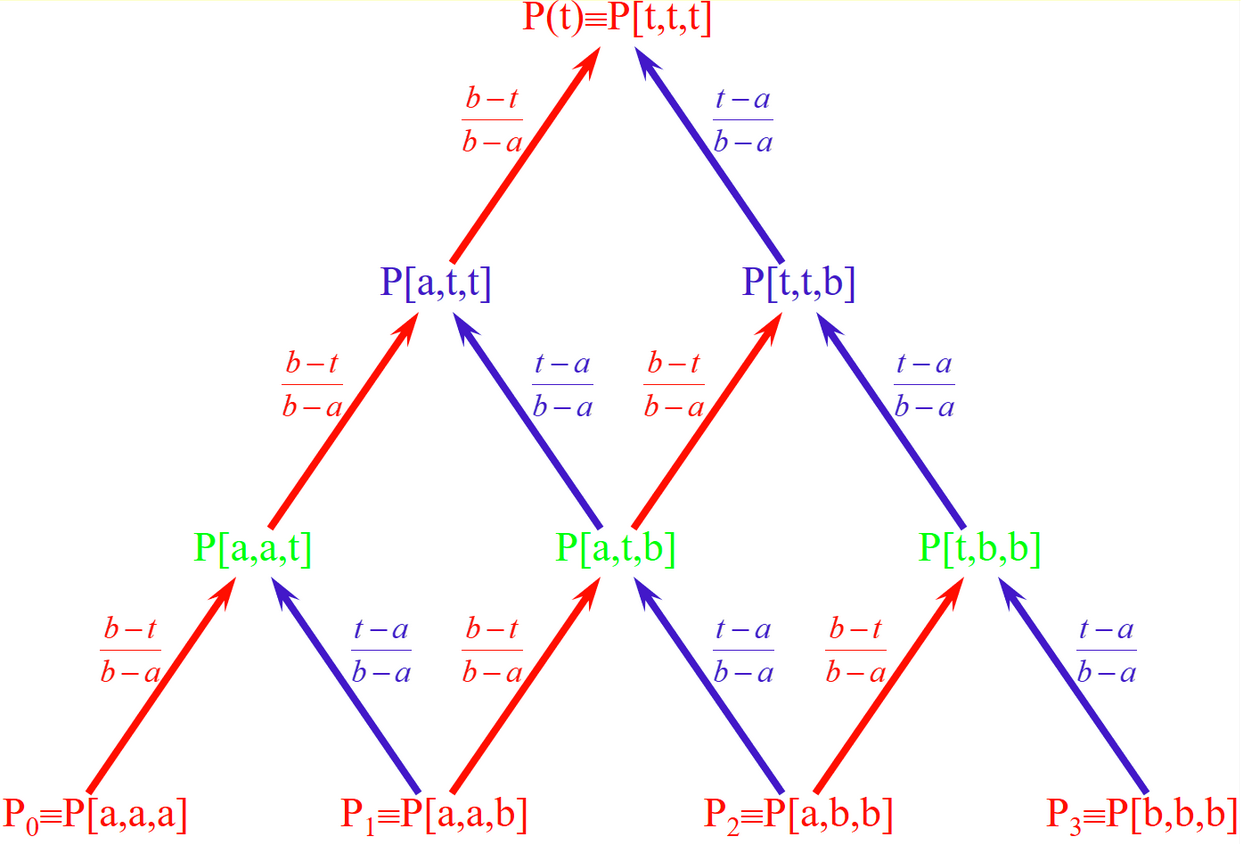
\includegraphics[width=\textwidth]{casteljau_construct_1}
				\caption{Algemene methode de Casteljau constructie.}
				\label{fig:casteljau_construct_1}
			\end{figure}
			\accentuate{Stel nu dat hij de punten op figuur \ref{fig:casteljau_construct_2} geeft (toevallig zelfde aantal punten). In dit geval komt $0$ overeen met $a$ en $1$ overeen met $b$. Hij zal enkel nog willekeurige $t-$waard geven. Vul het piramidaal schema in met deze $t$, en dan bekom je een gelijkaardige constructie zoals figuur \ref{fig:casteljau_construct_3}}.
			\begin{figure}[ht]
				\centering
				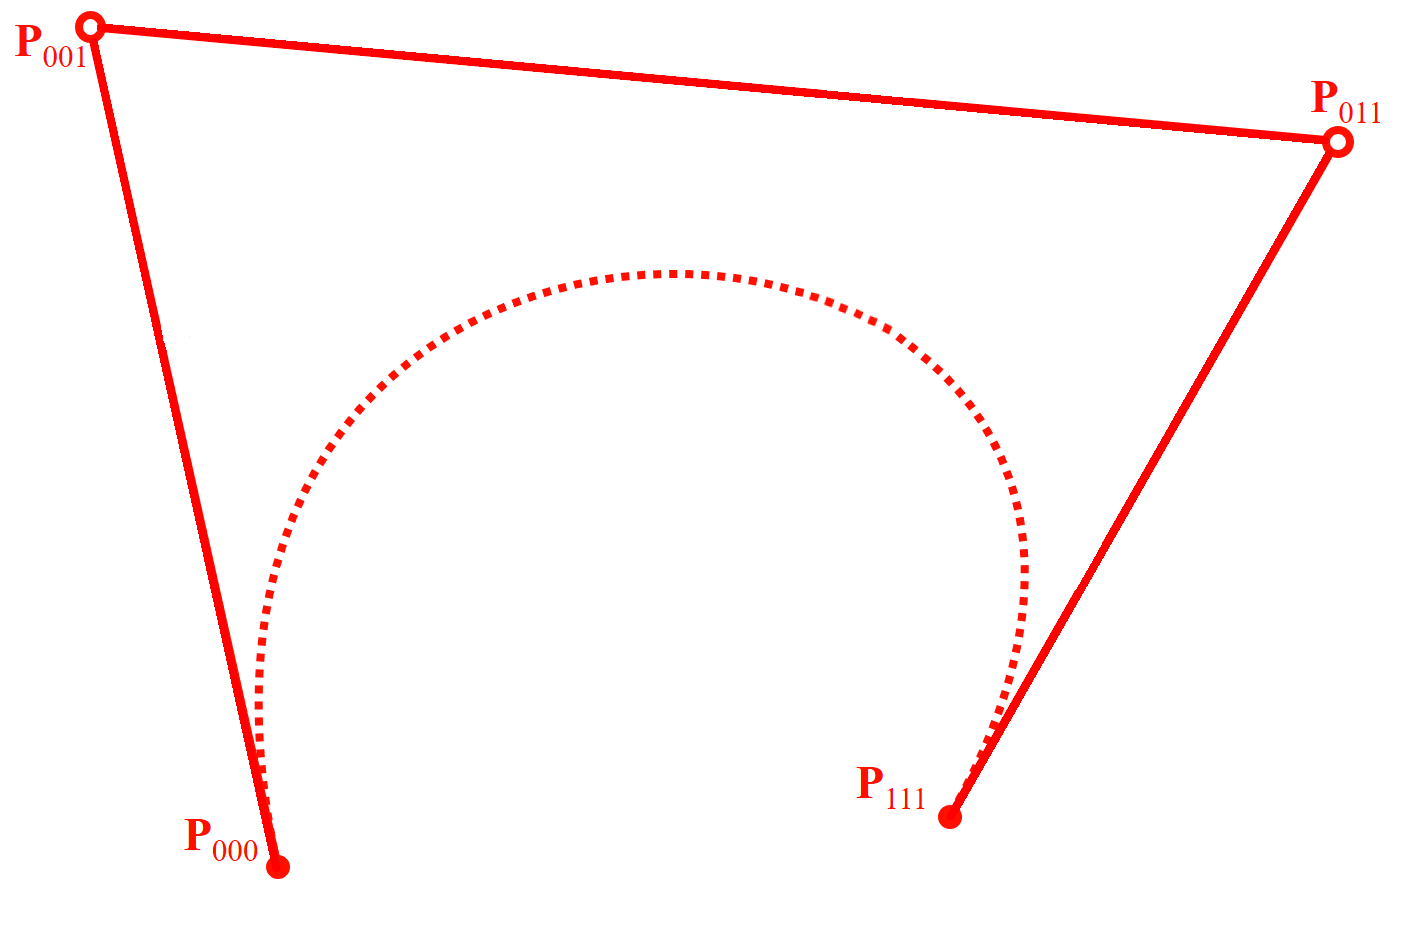
\includegraphics[width=0.6\textwidth]{casteljau_construct_2}
				\caption{Een willekeurige Bézier kromme.}
				\label{fig:casteljau_construct_2}
			\end{figure}
			\begin{figure}[ht]
				\centering
				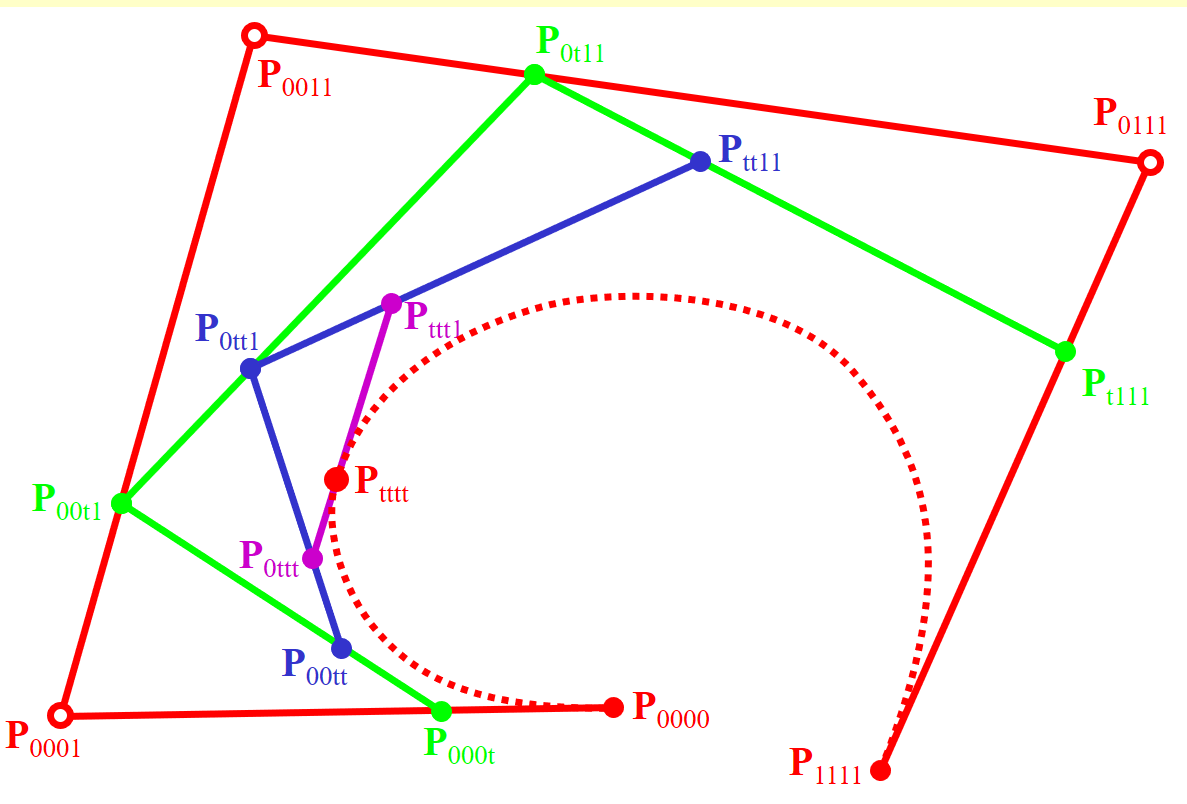
\includegraphics[width=0.6\textwidth]{casteljau_construct_3}
				\caption{de Casteljau constructie voor een willekeurige Bézier kromme.}
				\label{fig:casteljau_construct_3}
			\end{figure}
		\end{itemize}			
	}
	\vraag{\accentuate{(1)} verhoging van de graad van Bézier splines (in één enkele stap); voorafgaand moet het verband tussen de \textit{oude} en de \textit{nieuwe} controlepunten opgesteld worden (vermenigvuldiging met een specifieke matrix, cfr. theorieles)}{
		\begin{itemize} 
			Eerst algemene formule \accentuate{(niet te kennen)}:
			$$p[u_1, u_2, ... u_m] = \sum_{i_1 = 1}^{m}
			\sum_{\substack{i_2 = 1 \\ i_2 \neq i_1}}^{m}
			...
			\sum_{\substack{i_n = 1 \\ i_n \not\in \{i_1, ... i_{n}\}}}^{m}
			P[{u_i}_1, {u_i}_2, ..., {u_i}_n] \bigg/ \binom{m}{n}
			$$
			Een verhoging van de graad kan eenvoudig uitgevoerd worden met een matrix ($n + 1$ kolommen, $m + 1$ rijen), waarin de coëfficiënten van Pascal instaan. Hier uitgewerkt om een Bézier kromme van graad 3 te verhogen naar graad 6, in één enkele stap:
			$$
			\begin{pmatrix}
				1 & 0 & 0  & 0  \\ 
				1 & 1 & 0  & 0  \\ 
				1 & 2 & 1  & 0  \\ 
				1 & 3 & 3  & 1  \\ 
				0 & 4 & 6  & 4  \\ 
				0 & 0 & 10 & 10 \\ 
				0 & 0 & 0  & 20 
			\end{pmatrix}
			\rightarrow
			\begin{pmatrix}
				20 & 0  & 0 & 0 \\ 
				10 & 10 & 0 & 0 \\ 
				4  & 6  & 4 & 0 \\ 
				1  & 3  & 3 & 1 \\ 
				0  & 1  & 2 & 1 \\ 
				0  & 0  & 1 & 1 \\ 
				0  & 0  & 0 & 1 
			\end{pmatrix}
			\rightarrow
			\begin{pmatrix}
				20 & 0  & 0  & 0  \\ 
				10 & 10 & 0  & 0  \\ 
				4  & 12 & 4  & 0  \\ 
				1  & 9  & 9  & 1  \\ 
				0  & 4  & 12 & 4  \\ 
				0  & 0  & 10 & 10 \\ 
				0  & 0  & 0  & 20 
			\end{pmatrix}
			$$
			Deze matrix kan nu eenvoudig vermenigvuldigt worden met de kolommatrix van de punten:
			$$
			\begin{pmatrix}
				Q_{000000} (=Q_0) \\
				Q_{000001} (=Q_1)\\
				Q_{000011} (=Q_2)\\
				Q_{000111} (=Q_3)\\
				Q_{001111} (=Q_4)\\
				Q_{011111} (=Q_5)\\
				Q_{111111} (=Q_6)\\
			\end{pmatrix}
			= 
			\begin{pmatrix}
				20 & 0  & 0  & 0  \\ 
				10 & 10 & 0  & 0  \\ 
				4  & 12 & 4  & 0  \\ 
				1  & 9  & 9  & 1  \\ 
				0  & 4  & 12 & 4  \\ 
				0  & 0  & 10 & 10 \\ 
				0  & 0  & 0  & 20 
			\end{pmatrix}
			\cdot 
			\begin{pmatrix}
				P_{000} (=P_0)\\
				P_{001} (=P_1)\\
				P_{011} (=P_2)\\
				P_{111} (=P_3)\\
			\end{pmatrix}
			$$
			Elke kolom stelt één van de originele 4 punten voor. Een punt $P_i$ kan hieruit afgeleidt worden door op de $i$-de rij, de som van 
			de producten van het originele punt met de factor voor die kolom te berekenen, en deze som te delen door $\binom{m}{n}$. In dit geval is $m = 6$ en $n = 3$, zodat $\binom{6}{3} = \frac{6!}{3! 3!} = 20$. De zeven punten worden dus:
			\begin{itemize}
				\item $Q_0 = \frac{1}{20} (20P_0 + 0P_1  + 0P_2  + 0P_3) = P_0$
				\item $Q_1 = \frac{1}{20}(10P_0 + 10P_1 + 0P_2  + 0P_3) = \frac{1}{2}(P_0 + P_1)$ 
				\item $Q_2 = \frac{1}{20}(4P_0  + 12P_1 + 4P_2  + 0P_3) = \frac{1}{5}(P_0  + 3P_1 + P_2)$
				\item $Q_3 = \frac{1}{20}(1P_0  + 9P_1 + 9P_2  + 1P_3) = \frac{1}{20}(P_0 + 9P_1  + 9P_2 + P_3)$
				\item $Q_4 = \frac{1}{20}(0P_0  + 4P_1 + 12P_2  + 4P_3) = \frac{1}{5}(P_1  + 3P_2 + P_3)$
				\item $Q_5 = \frac{1}{20}(0P_0  + 0P_1 + 10P_2  + 10P_3) = \frac{1}{2}(P_2 + P_3)$
				\item $Q_6 = \frac{1}{20}(0P_0  + 0P_1 + 0P_2  + 20P_3) = P_3$
			\end{itemize}		
		\end{itemize}}
	\vraag{\accentuate{(2)} verhoging van de graad van Bézier splines (\textit{stapsgewijs}: één graad verhogen per stap)}{
		\begin{itemize} 
			\item Slechts één graad verhogen per stap is heel eenvoudig:
			      $$Q_k = \frac{k}{n + 1}P_{k - 1} + \frac{n + 1 - k}{n + 1}P_k$$
			      Stel een bézierkromme van de 3de graad met punten $P_{000}, P_{001}, P_{011}$ en $P_{111}$.
			      			
			      De nieuwe punten van de bézierkromme van de 4de graad worden dan:
			      \begin{itemize}
			      	\item $Q_{0000} =\frac{3 + 1 - 0}{3 + 1}P_{00} = P_{000}$
			      	\item $Q_{0001} = \frac{1}{4}P_{000} + \frac{4 - 1}{4}P_{001} = \frac{1}{4}P_{000} + \frac{3}{4}P_{001}$
			      	\item $Q_{0011} = \frac{1}{2}P_{001} + \frac{1}{2}P_{011}$
			      	\item $Q_{0111} = \frac{3}{4}P_{011} + \frac{1}{4}P_{111}$
			      	\item $Q_{1111} = P_{111}$
			      \end{itemize}
			      Het punt $Q_{0001}$ ligt bijvoorbeeld op $t = 0.75$ voor het lijnstuk $[P_{000}P_{001}]$.
		\end{itemize}}

	\vraag{\accentuate{(3,4)} segmentering (subdivisie) van Bézier krommen (eventueel meerdere segmenten in één enkele stap)}
		{
			\begin{itemize} 
				\item \accentuate{Als je een de Casteljau constructie toepast op een Bézier kromme, introduceer je hulppunten, die perfect kunnen dienen als de nieuwe punten van twee of meerdere bézierkrommen. Bekijk voorbeeld \ref{fig:subdivision_1}, waarbij de Bézierkromme gegeven wordt door de punten $(P_{0000}, P_{0001},$ $P_{0011}, P_{0111}, P_{1111})$. Het kan onmiddelijk gesegmenteerd worded in twee bézier krommen, respectievelijk bepaald door $(P_{0000},P_{000t},P_{00tt},P_{0ttt},P_{tttt})$ en $(P_{tttt},P_{ttt1},P_{tt11},P_{t111},P_{1111})$. Het is ook mogelijk om kubieke Bézierkrommem in meerdere segmenten op te splitsen, zoals \ref{fig:subdivision_2}, die respectievelijk segmenten bepalen door $(P_{000}, P_{00s}, P_{0ss}, P_{sss})$, $(P_{sss}, P_{sst}, P_{stt}, P_{ttt})$ en $(P_{ttt}, P_{tt1}, P_{t11}, P_{111})$. }
				\begin{figure}[ht]
					\centering
					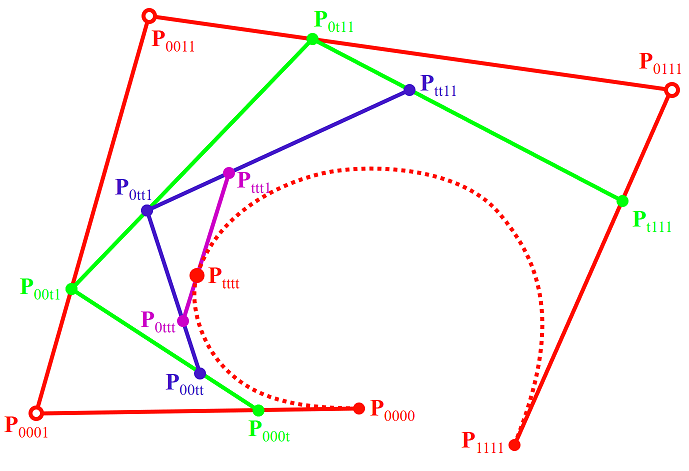
\includegraphics[width=\textwidth]{subdivision_1}
					\caption{Een bézierkromme van graad vier.}
					\label{fig:subdivision_1}
				\end{figure}
				\begin{figure}[ht]
					\centering
					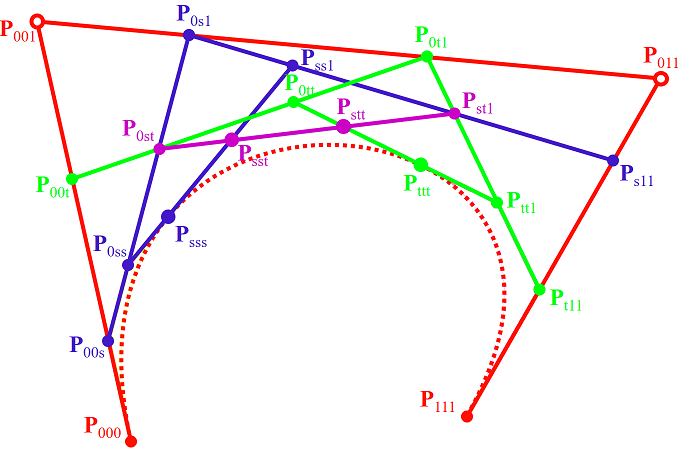
\includegraphics[width=\textwidth]{subdivision_2}
					\caption{Een kubieke bézierkromme van graad drie.}
					\label{fig:subdivision_2}
				\end{figure}
			
			\end{itemize}
		}
	\vraag{\accentuate{(9-10,14-16)} constructie van de \textit{kromtecirkel} in een punt van een Bézier kromme}
	{
		\begin{itemize} 
			\item \accentuate{Algemene methode om een kromtecirkel te berekenen in een punt van een Bézier kromme wordt weergegeven op figuur \ref{fig:kromtecirkel}. De kromming van een Bézier kromme wordt bepaald door de hulppunten van de laatste 2 iteraties van het de Casteljau proces. Eerst moet dus een de Casteljau constructie uitgevoerd worden op de Bézier kromme voor het opgegeven punt $t$. De straal $R$ van de kromtecirkel wordt gegeven door $$R = \frac{3\Delta^2}{4\delta}$$
			Het volgende proces kan op twee manieren uitgevoerd worden, hier doe ik het voor de controlepunten $(P_{00t}, P_{0tt})$, maar zou evengoed gelden voor de controlepunten $(P_{tt1}, P_{t11})$. De afstand van $P_{ttt}$ tot $P_{0tt}$ noemen we $\Delta_0$ (is vrij onbelangrijk, maar toch vermeld ik het omdat het op de figuur staat). Het lijnstuk dat samenvallend is met $|P_{ttt}P_{0tt}|$ moet doorgetrokken worden, zodanig dat er een rechte hoek gemaakt kan worden tussen het eindpunt van dit lijnstuk en het punt $P_{00t}$. De afstand van $P_{00t}$ en dit eindpunt noemen we $\delta_0$. Nu kunnen we een lijnstuk, loodrecht op het lijnstuk $|P_{0tt}P_{tt1}|$ en door het punt $P_{ttt}$ met lengte $\frac{4}{3} \delta_0$ tekenen. Op dit moment kan er vanuit $P_{0tt}$ een lijnstuk getrokken worden tot aan het einde van het vorige lijnstuk, gevolgd door een ander lijnstuk, loodrecht met het vorige lijnstuk, zodanig dat het kruist met het verlengde van het lijnstuk door $P_{ttt}$. Deze kruising is het middelpunt van de cirkel. De afstand van dit middelpunt tot $P_{ttt}$ is de straal $R$ van de cirkel.
			}
			\begin{figure}[ht]
				\centering
				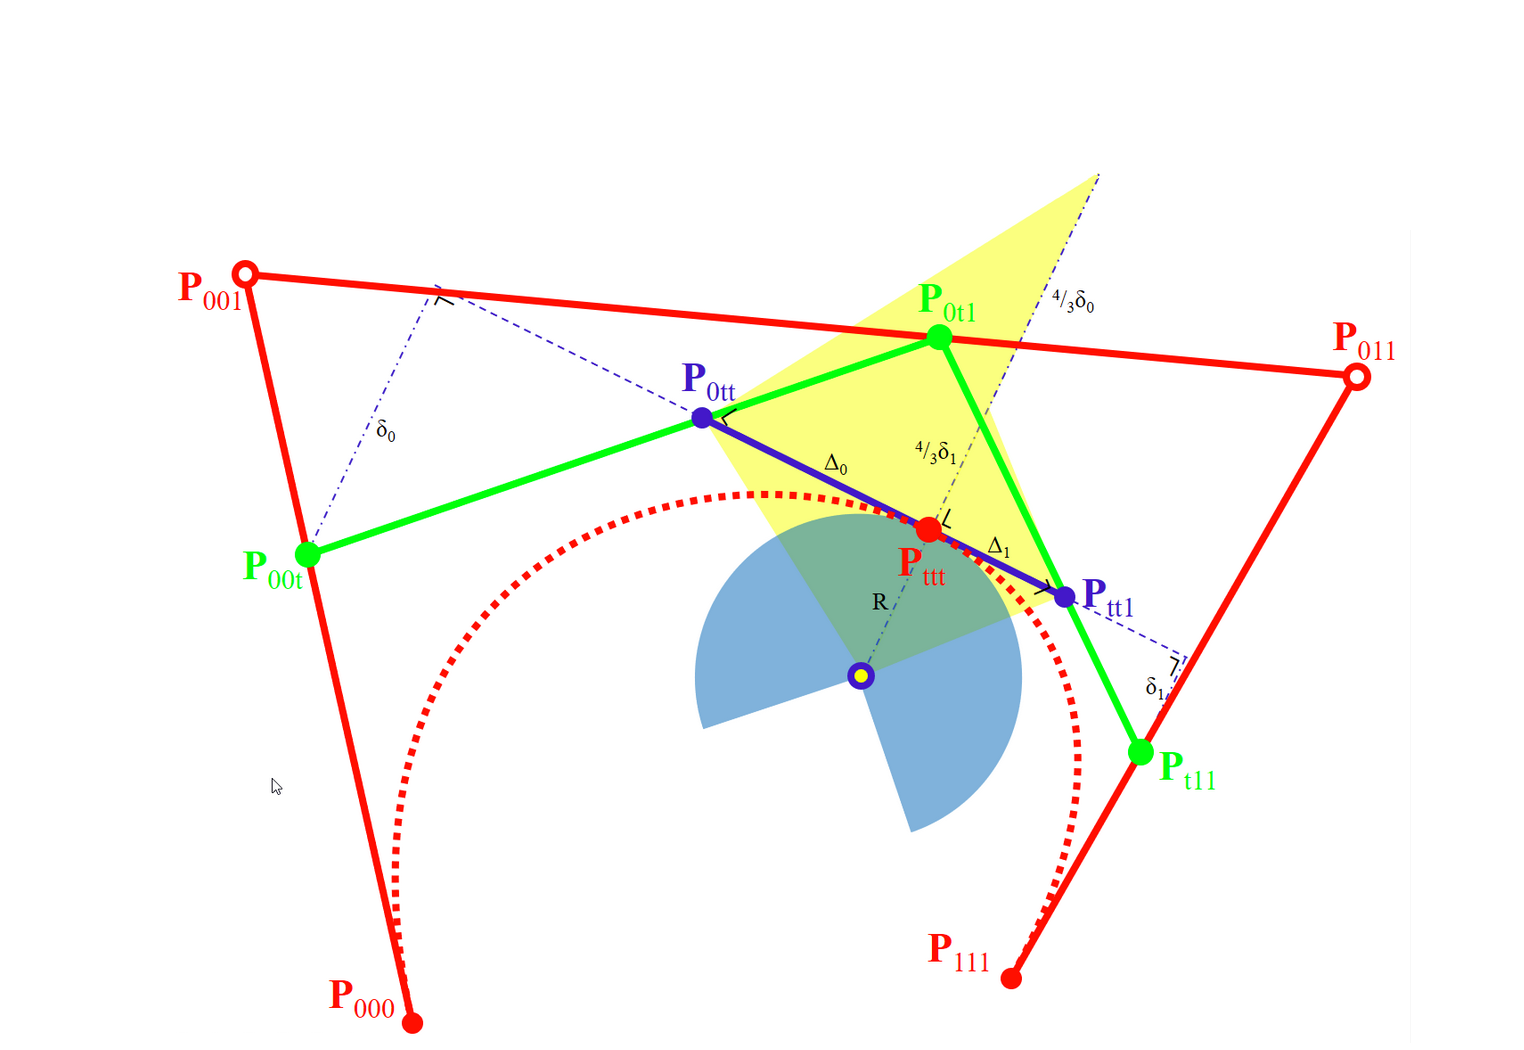
\includegraphics[width=\textwidth]{kromtecirkel}
				\caption{De kromtecirkel door het punt $P_{ttt}$.}
				\label{fig:kromtecirkel}
			\end{figure}
		\end{itemize}
			
		}
	\vraag{\accentuate{(5-7,9-11)} constructie van de \textit{Bézier representatie} van een (polynomiale) NURBS}{
		\begin{itemize}
			\item De knooppunten van de B-spline worden datapunten van de Bézier-representatie. Deze vraag wordt opgelost met het voorbeeld op figuur \ref{fig:bezier_repr_polynomiale_nurbs_1}.
			\begin{figure}[ht]
				\centering
				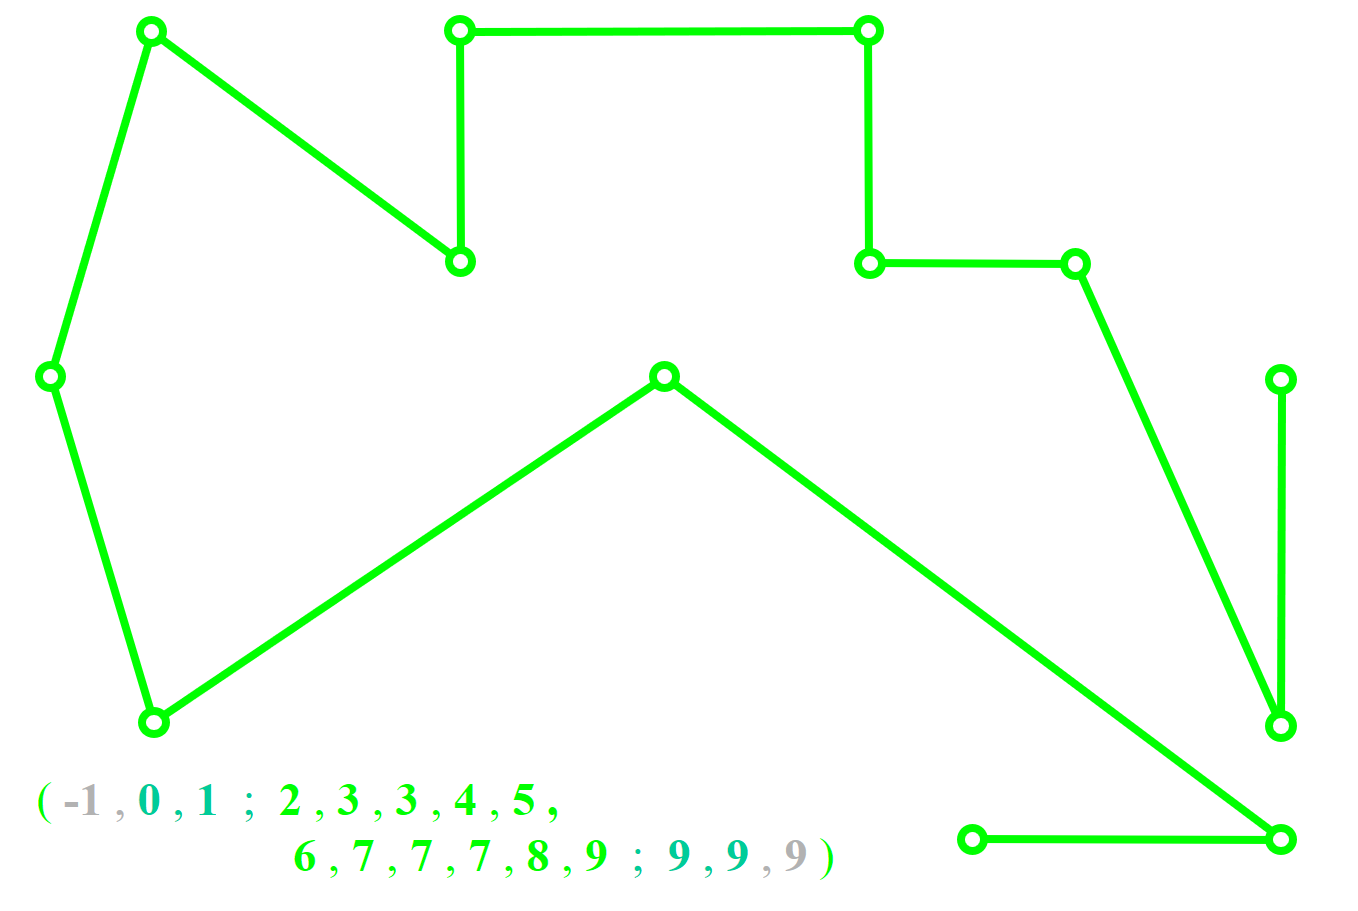
\includegraphics[width=0.5\textwidth]{bezier_repr_polynomiale_nurbs_1}	
				\caption{Fase 1 bézier representatie van een polynomiale NURBS}
				\label{fig:bezier_repr_polynomiale_nurbs_1}
			\end{figure}

			De knopenvector wordt gegeven: $(-1, 0, 1 ; 2, 3, 3, 4, 5, 6, 7, 7, 7, 8, 9 ; 9, 9, 9)$. Wat meteen opvalt is dat er 7 (waarvan sommige hogere multipliciteit) reële knooppunten zijn, wat betekent dat de resulterende bézier spline 6 segmenten zal bevatten. Schrijf eerst de blossomnotatie van elk knooppunt, zoals weergegeven op figuur \ref {fig:bezier_repr_polynomiale_nurbs_2}.
			\begin{figure}[ht]
				\centering
				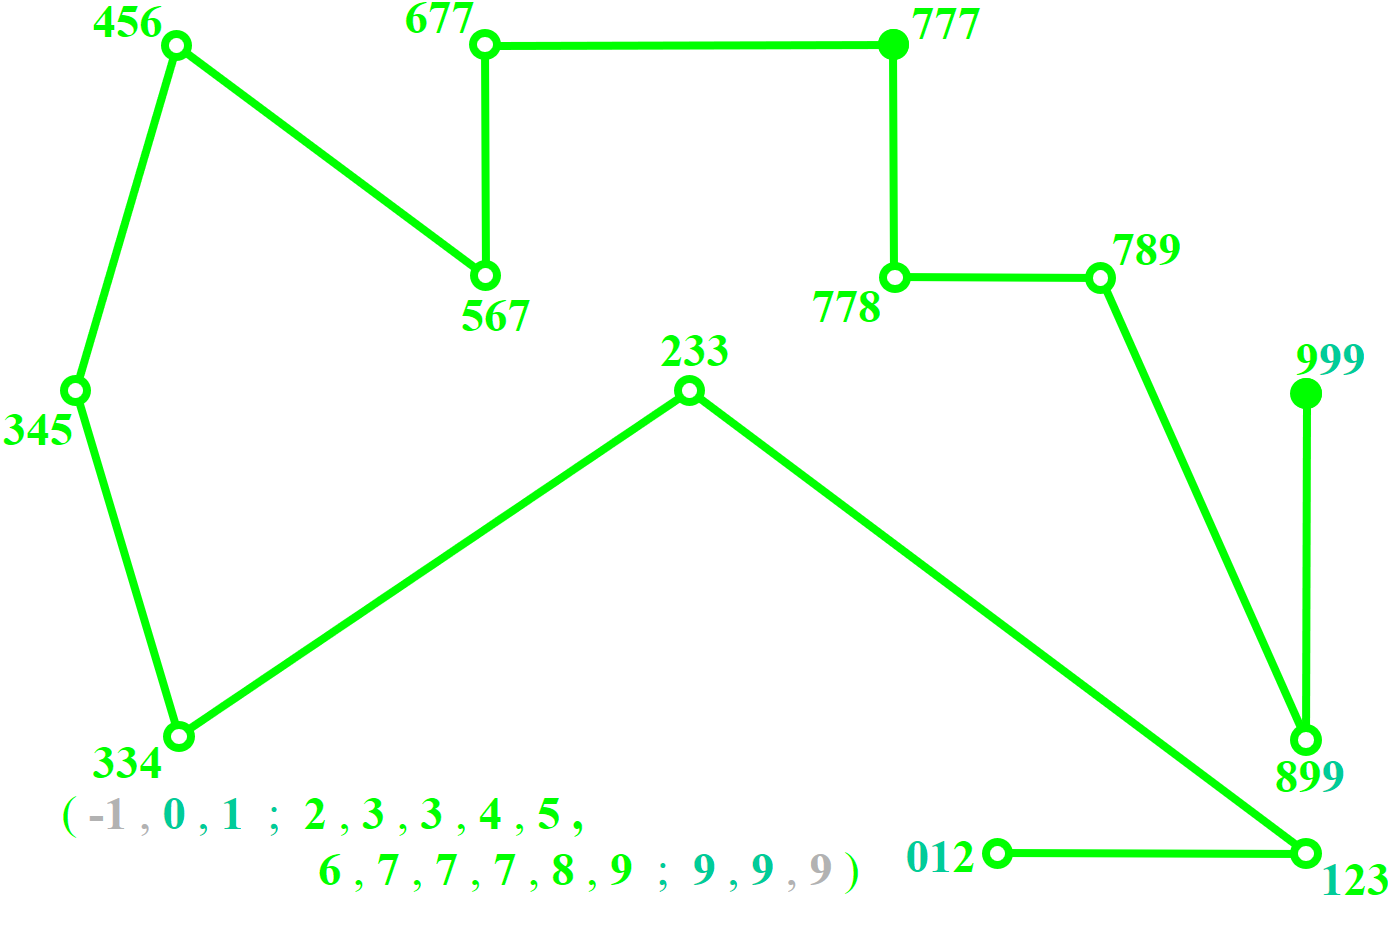
\includegraphics[width=0.5\textwidth]{bezier_repr_polynomiale_nurbs_2}	
				\caption{Fase 2 bézier representatie van een polynomiale NURBS}
				\label{fig:bezier_repr_polynomiale_nurbs_2}
			\end{figure}

			Via de multilineariteit eigenschap kan men nieuwe punten introduceren. (\accentuate{herhaling op figuur \ref{fig:multilineariteit}})
			\begin{figure}[ht]
				\centering
				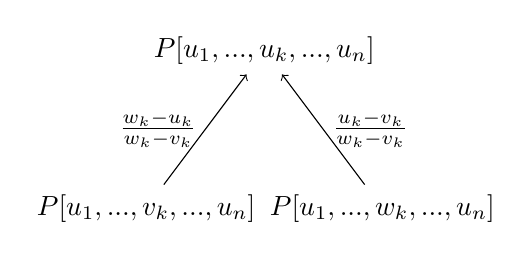
\begin{tikzpicture}
					\node (x) at (0, 0) {$P[u_1,...,v_k,...,u_n]$};
					\node (z) at (1.5, 2) {$P[u_1,...,u_k,...,u_n]$};
					\node (y)at (3, 0) {$P[u_1,...,w_k,...,u_n]$};

					\draw[->] (x) -- node[xshift=-0.6cm]{$\frac{w_k - u_k}{w_k - v_k}$} (z);
					\draw[->] (y) -- node[xshift=0.6cm]{$\frac{u_k - v_k}{w_k - v_k}$} (z);
				\end{tikzpicture}
				\caption{multilineariteit.}
				\label{fig:multilineariteit}
			\end{figure}	

			Bijvoorbeeld: tussen punt 012 en 123 moeten nog twee hulppunten komen: 112 en 122. Stel in het diagram $u_k = 1, v_k = 0$ en $w_k = 2$. dan krijgen we
			$$P[1,1,2] = \frac{2}{3}P[0,1,2] + \frac{1}{3}P[1,2,3]$$
			of anders gezegd: het punt 112 ligt op $t = 1/3$ voor het lijnstuk $[P[0,1,2]P[1,2,3]]$.
			Analoog voor $u_k = 2, v_k = 0$ en $w_k = 2$, dan krijgen we
			$$P[1,2,2] = \frac{1}{3}P[0,1,2] + \frac{2}{3}P[1,2,3]$$
			of anders gezegd: het punt 122 ligt op $t = 2/3$ voor het lijnstuk  $[P[0,1,2]P[1,2,3]]$.
			Als je dit zou doen voor punten 123 en 233, dan zou je 
			$$P[2, 2, 3] = \frac{1}{2}P[1,2,3] + \frac{1}{2}P[2,3,3]$$
			krijgen, zodat het punt 223 mooi in het midden van het lijnstuk $[P[1,2,3]P[2,3,3]]$ ligt. Een leuke eigenschap is, dat als de knopenvector geen gaten vertoond, dat het lijnstuk altijd mooi opgesplitst wordt. Als je op een lijnstuk dan 2 hulppunten moet introduceren, zal het eerste punt op $1/3$ van het lijnstuk liggen, en het tweede punt op $2/3$. Als je 3 hulppunten moet introduceren, zal het eerste punt op $1/4$ van het lijnstuk liggen, enz... Een voorbeeld van een knopenvector met gaten, waardoor je dus best manueel uitrekend, is $(0, 1, 3 ; 4, 6 ; 7, 9, 10)$. Alle nieuwe hulppunten kunnen zo berekend worden, en is te zien op figuur \ref{fig:bezier_repr_polynomiale_nurbs_3}.
			\begin{figure}[ht]
				\centering
				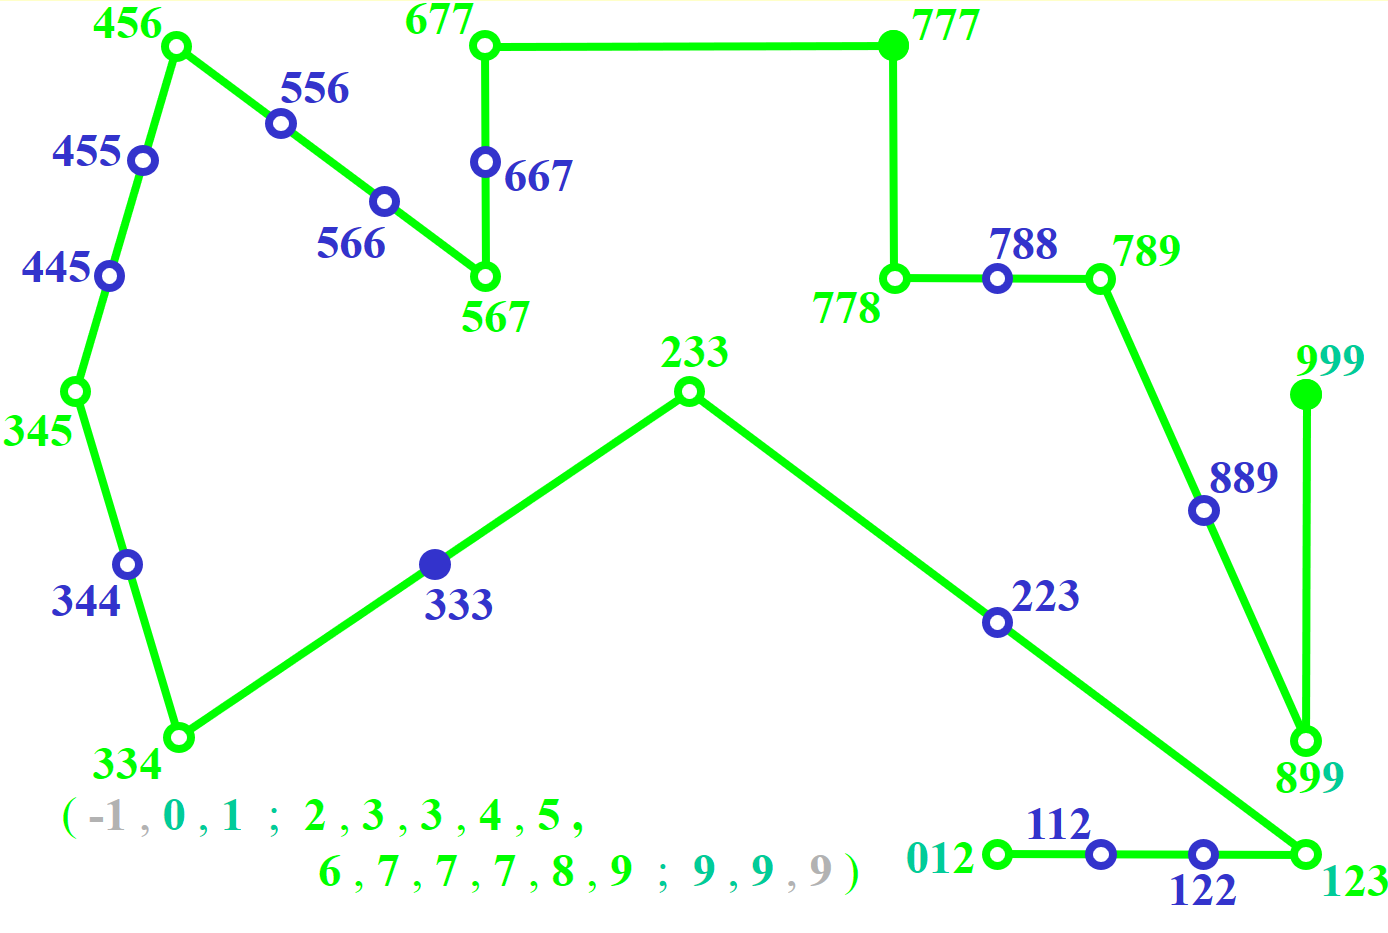
\includegraphics[width=0.5\textwidth]{bezier_repr_polynomiale_nurbs_3}	
				\caption{Fase 3 bézier representatie van een polynomiale NURBS}
				\label{fig:bezier_repr_polynomiale_nurbs_3}
			\end{figure}

			Punten waarvan slechts 1 argument van de blossomnotatie verschillen, kunnen geïnterpoleerd worden. Teken een lijnstuk door elk paar punten waarvoor dit van toepassing is. Op figuur \ref{fig:bezier_repr_polynomiale_nurbs_4} wordt dit uitgewerkt, samen met het introduceren van de nieuwe hulppunten.
			\begin{figure}[ht]
				\centering
				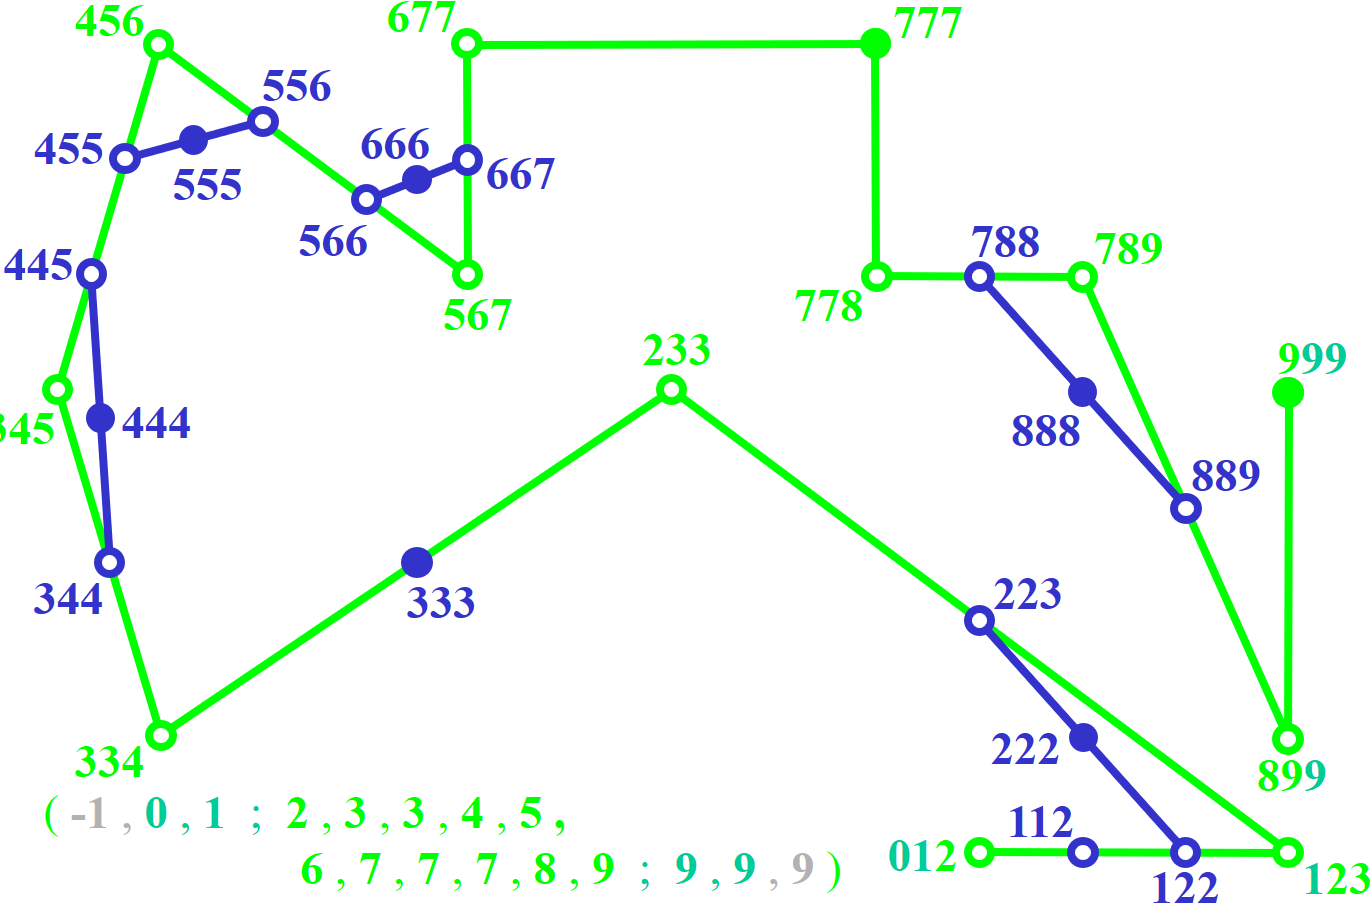
\includegraphics[width=0.5\textwidth]{bezier_repr_polynomiale_nurbs_4}	
				\caption{Fase 4 bézier representatie van een polynomiale NURBS}
				\label{fig:bezier_repr_polynomiale_nurbs_4}
			\end{figure}

			Tot slot moeten nog enkel de punten verbonden worden waarvan de blossomnotatie bestaat uit een herhaling van slechts één argument. In dit voorbeeld zijn dat de punten 222, 333, 444, 555, 666, 777, 888 en 999. Zoek eerst in de knopenvector op of er knooppunten zijn met een hogere multipliciteit. \accentuate{De continuïteit in een knooppunt horend bij een knoop met multipliciteit $\mu$ wordt gegeven door $C^{k - 1 - \mu}$}.
			
			Het knooppunt 3 heeft een multipliciteit van 2, zodat slechts $C^{4 - 1 - 2} = C^1$ continuïteit voldaan is. Het knooppunt 7 heeft een multipliciteit van 3, zodat daar slechts $C^0$ voldaan is. Dit is belangrijk bij het tekenen van de kromme, zoals te zien op figuur \ref{fig:bezier_repr_polynomiale_nurbs_5}.
			\begin{figure}[ht]
				\centering
				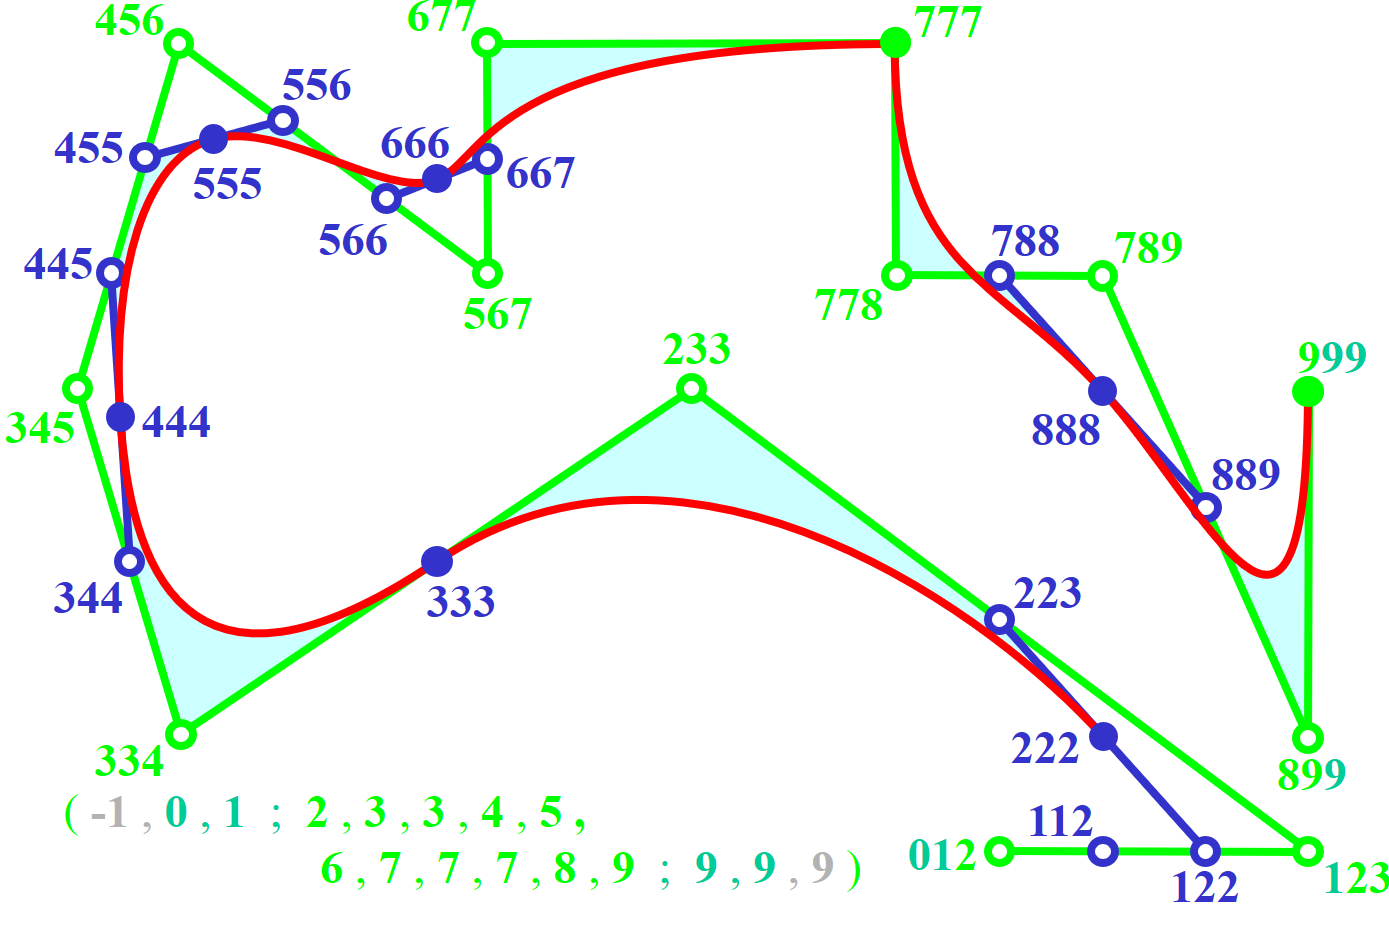
\includegraphics[width=0.5\textwidth]{bezier_repr_polynomiale_nurbs_5}	
				\caption{Fase 5 bézier representatie van een polynomiale NURBS}
				\label{fig:bezier_repr_polynomiale_nurbs_5}
			\end{figure}
		\end{itemize}}
	\vraag{\accentuate{(6-10)} constructie van controlepunten na toevoeging van één of meerdere \textit{reële} knopen in de knopenvector van een (polynomiale) NURBS (zonder over te gaan op de Bézier representatie)}{\begin{itemize} \item \todo{oplossen} \end{itemize}}
	\vraag{\accentuate{(10)} constructie van controlepunten na toevoeging van één of meerdere \textit{virtuele} knopen in de knopenvector van een (polynomiale) NURBS (zonder over te gaan op de Bézier representatie)}{\begin{itemize} \item \todo{oplossen} \end{itemize}}
	\vraag{\accentuate{(11)} berekening en constructie van de controlepunten van de \textit{open-uniforme} representatie van een (polynomiale) NURBS met een \textit{uniforme} knopenvector}{\begin{itemize} \item \todo{oplossen} \end{itemize}}
	\vraag{\accentuate{(12,19)} berekening en constructie van de controlepunten van de \textit{uniforme} representatie van een polynomiale of rationale NURBS met een \textit{open-uniforme} knopenvector}{\begin{itemize} \item \todo{oplossen} \end{itemize}}
	\vraag{\accentuate{(12)} de Boor constructie (van een punt met specifieke parameterwaarde) van een (polynomiale) NURBS}{\begin{itemize} \item \todo{oplossen} \end{itemize}}
	\vraag{\accentuate{(13)} constructie van de \textit{hodograaf} van een Bézier kromme of spline}{\begin{itemize} \item \todo{oplossen} \end{itemize}}
	\vraag{\accentuate{(13-16)} vaststellen van de continuïteit in de knooppunten van Bézier splines (\textit{stelling van Stärk})}
	{
		\begin{itemize} 
		\item \textbf{Stelling van Stärk:} Men bereikt $C^k$ continuïteit indien de blossomargumenten voor elk van de $2k$ naburige controlepunten hetzelfde punt in de ruimte oplevert, of men nu de argumenten evalueert in de blossompolynoom van het ene segment, of in de blossompolynoom van het andere segment. 
		\item Stel een linkersegment met data- en controlepunten $P[a, a, a], P[a, a, b], P[a, b, b]$ en $P[b, b, b]$, en een rechtersegment, bepaald door $Q[b, b, b], Q[b, b, c], Q[b, c, c]$ en $Q[c, c, c]$ met gemeenschappelijk punt $P[b, b, b] \equiv Q[b, b, b]$. Aangezien we dit gemeenschappelijk punt hebben is $C^0$ continuïteit voldaan. Om $C^1$ continuïteit te bereiken moet, indien men de argumenten van controlepunt $P[a, b, b]$ van het linkersegment evalueert in de blossom van het rechtersegment, dit een punt $Q[a, b, b]$ oplevern dat samenvalt met $P[a, b, b]$
			
		\end{itemize}
	}
	\vraag{\accentuate{(17)} constructie van de controlepunten van de \textit{uniforme} Lagrange representatie van een Lagrange geïnterpoleerde kromme met \textit{niet-uniforme} knopenvector; schematisch aantonen hoe de berekening van de Bézier representatie van deze kromme zou kunnen uitgevoerd worden (ondermeer opstellen van de \textit{inverse} van de Bézier basismatrix).}{
		\begin{itemize} 
			\item Veronderstel de niet-uniforme knopenvector $\{0, 3, 6, 12\}$ en volgende figuur (\accentuate{afbeelding kan niet volledig kloppen, dient enkel als illustratie}):
			
			\begin{figure}[h]
				\centering
				\begin{tikzpicture}[every node/.style={circle, fill=red},
									label/.style={fill=none}]
					\node (p0) at (0, 0) {};
					\node[label] at (-0.5, 0) {$P_{0}$};
					\node (p1) at (3, 3) {};
					\node[label] at (3, 3.5) {$P_{1}$};
					\node (p2) at (4, -0.1) {};
					\node[label] at (4, 0.4) {$P_{2}$};
					\node (p3) at (9, -0.2) {};
					\node[label] at (9,0.3) {$P_{3}$};

					\draw[red] plot [smooth, tension=1.4] coordinates {(0, 0) (3, 3) (4, -0.1) (9, -0.2)};
				\end{tikzpicture}
			\end{figure}
			De uniforme knopenvector bekomt men door van de originele niet-uniforme knopenvector een rekenkundige rij te maken: $\{0, 4, 8, 12\}$. Punt $P_0$ en $P_{3}$ blijven ongewijzigd. Punten $P_1$ en $P_2$ moeten opnieuw berekend worden. Teken eerst de lijnstukken $[P_0P_1], [P_1P_2]$ en $[P_2P_3]$. 

			\begin{figure}[h]
				\centering
				\begin{tikzpicture}[every node/.style={circle, fill=red},
					label/.style={fill=none}]

					\node (p0) at (0, 0) {};
					\node[label] at (-0.5, 0) {$P_{0}$};
					\node (p1) at (3, 3) {};
					\node[label] at (3, 3.5) {$P_{1}$};
					\node (p2) at (4, -0.1) {};
					\node[label] at (4, 0.4) {$P_{2}$};
					\node (p3) at (9, -0.2) {};
					\node[label] at (9,0.3) {$P_{3}$};


					\draw[red] plot [smooth, tension=1.4] coordinates {(0, 0) (3, 3) (4, -0.1) (9, -0.2)};

					\draw (p0) -- (p1);
					\draw (p1) -- (p2);
					\draw (p2) -- (p3);
				\end{tikzpicture}
			\end{figure}
			In de niet-uniforme knopenvector wordt $P_1$ bereikt voor $t = 3$. Het punt $P_1$ moet echter in de uniforme knopenvector bereikt worden voor $t = 4$. Analoog voor het punt $P_2$, die nu bereikt moet worden voor $t = 8$. Gebruik van het piramidaal schema geeft de exacte posities van deze punten. \accentuate{Algemeen:}
			\begin{figure}[ht]
				\centering
				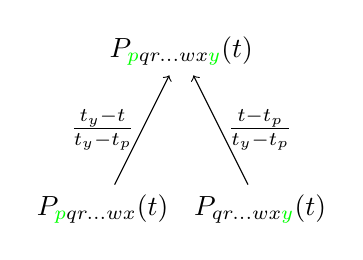
\begin{tikzpicture}
					\node (x) at (0, 0) {$P_{{\color{green}p}qr...wx}(t)$};
					\node (z) at (1, 2) {$P_{{\color{green}p}qr...wx{\color{green}y}}(t)$};
					\node (y)at (2, 0) {$P_{qr...wx{\color{green}y}}(t)$};

					\draw[->] (x) -- node[xshift=-0.5cm]{$\frac{t_y - t}{t_y - t_p}$} (z);
					\draw[->] (y) -- node[xshift=0.5cm]{$\frac{t - t_p}{t_y - t_p}$} (z);
				\end{tikzpicture}
			\end{figure}

			Toegepast voor $t = 4, t_0 = 0, t_1 = 3, t_2 = 6$ en $t_3 = 12$:
			\begin{figure}[ht]
				\centering
				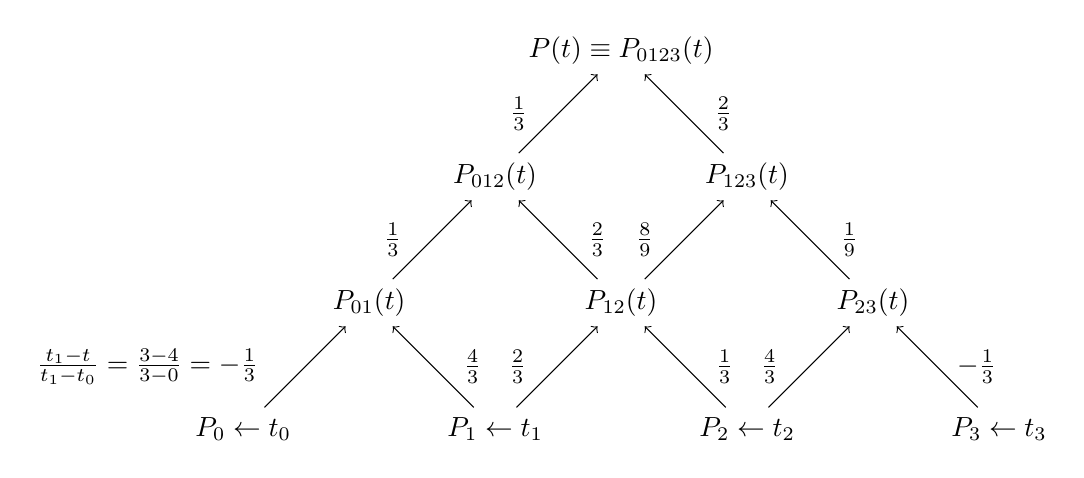
\begin{tikzpicture}[scale=0.8]
					\node (p0) at (0, 0) {$P_0 \leftarrow t_0$};
					\node (p01) at (2, 2) {$P_{01}(t)$};
					\node (p1) at (4, 0) {$P_1 \leftarrow t_1$};
					\node (p12) at (6, 2) {$P_{12}(t)$};
					\node (p2) at (8, 0) {$P_2 \leftarrow t_2$};
					\node (p23) at (10, 2) {$P_{23}(t)$};
					\node (p3) at (12, 0) {$P_3 \leftarrow t_3$};
				

					\node (p012) at (4, 4) {$P_{012}(t)$};
					\node (p123) at (8, 4) {$P_{123}(t)$};

					\node (p0123) at (6, 6) {$P(t) \equiv P_{0123}(t)$};

					\draw[->] (p0) -- node[xshift=-2cm]{$\frac{t_1 - t}{t_1 - t_0} = \frac{3 - 4}{3 - 0} = -\frac{1}{3}$} (p01);
					\draw[->] (p1) -- node[xshift=0.5cm]{$\frac{4}{3}$} (p01);

					\draw[->] (p1) -- node[xshift=-0.5cm]{$\frac{2}{3}$} (p12);
					\draw[->] (p2) -- node[xshift=0.5cm]{$\frac{1}{3}$} (p12);

					\draw[->] (p2) -- node[xshift=-0.5cm]{$\frac{4}{3}$} (p23);
					\draw[->] (p3) -- node[xshift=0.5cm]{$-\frac{1}{3}$} (p23);

					\draw[->] (p01) -- node[xshift=-0.5cm]{$\frac{1}{3}$} (p012);
					\draw[->] (p12) -- node[xshift=0.5cm]{$\frac{2}{3}$} (p012);
					\draw[->] (p12) -- node[xshift=-0.5cm]{$\frac{8}{9}$} (p123);
					\draw[->] (p23) -- node[xshift=0.5cm]{$\frac{1}{9}$} (p123);

					\draw[->] (p012) -- node[xshift=-0.5cm]{$\frac{1}{3}$} (p0123);
					\draw[->] (p123) -- node[xshift=0.5cm]{$\frac{2}{3}$} (p0123);
				\end{tikzpicture}
			\end{figure}

			Hieruit kunnen eenvoudig alle (hulp)punten afgeleidt worden \accentuate{($P_{01}$ ligt op $4/3$ van het lijnstuk $[P_0P_1$], $P_{123}$ ligt op $1/9$ van het lijnstuk $[P_{12}P_{23}]$)}:

			\begin{figure}[ht]
				\centering
				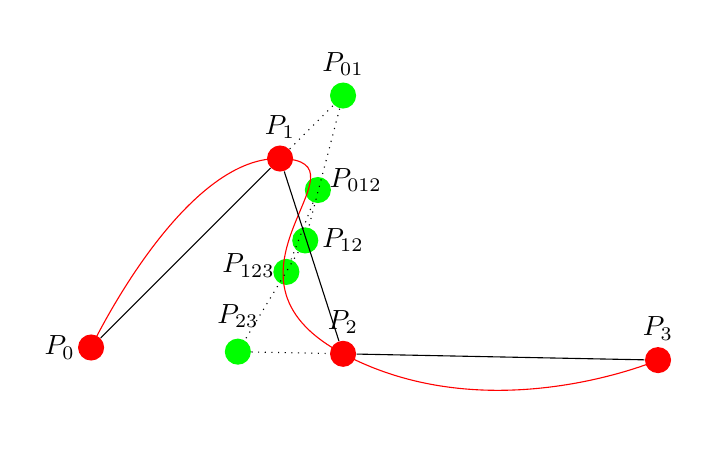
\begin{tikzpicture}[every node/.style={circle, fill=red},
					label/.style={fill=none}, 
					new/.style={fill=green},
					scale=0.8]

					\node (p0) at (0, 0) {};
					\node[label] at (-0.5, 0) {$P_{0}$};

					\node (p1) at (3, 3) {};
					\node[label] at (3, 3.5) {$P_{1}$};

					\node[new] (p01) at (4, 4) {};
					\node[label] at (4,4.5) {$P_{01}$};

					\node[new] (p23) at (2.33, -0.066) {};
					\node[label] at (2.33,0.5) {$P_{23}$};

					\node[new] (p12) at (3.4, 1.7) {};
					\node[label] at (4,1.7) {$P_{12}$ };

					\node[new] (p012) at (3.6, 2.5) {};
					\node[label] at (4.2,2.66) {$P_{012}$};

					\node (p2) at (4, -0.1) {};
					\node[label] at (4, 0.4) {$P_{2}$};

					\node[new] (p123) at (3.1, 1.2) {};
					\node[label] at (2.5,1.3) {$P_{123}$};

					\node (p3) at (9, -0.2) {};
					\node[label] at (9,0.3) {$P_{3}$};


					\draw[red] plot [smooth, tension=1.4] coordinates {(0, 0) (3, 3) (4, -0.1) (9, -0.2)};

					\draw (p0) -- (p1);
					\draw (p1) -- (p2);
					\draw (p2) -- (p3);

					\draw[dotted] (p1) -- (p01);
					\draw[dotted] (p01) -- (p12);

					\draw[dotted] (p12) -- (p23);
					\draw[dotted] (p23) -- (p2);

					\draw[dotted] (p012) -- (p123);
				\end{tikzpicture}
			\end{figure}

			\todo{figuur ontbreekt $P_{0123}$ aangezien deze figuur niet klopt. Je kan zien dat het lijnstuk $[P_{012}P_{123}]$ geen punt van de kromme heeft, dit komt puur door het feit dat de kromme niet juist getekend is.}

			\item De matrix voor een Bézierkromme van willekeurige graad $n$ kan als volgt opgesteld worden:
				\begin{enumerate}
					\item Construeer de driehoek van Pascal, in de linkerbovenhoek van een $(n + 1) \cdot (n + 1)$ matrix, vertrekkend van de rechterbovenhoek. De overige coëfficiënten blijven nul.
					\item Vermenigvuldig alle coëfficiënten van kolom $j$, met de coëfficiënt in rij $j$ van de eerste kolom.
					\item Keer het teken om van alle coëfficiënten op de even nevendiagonalen. 
				\end{enumerate}
				Toegepast op de figuur \accentuate{($n = 3$ aangezien 4 datapunten)}:
				$$
				\begin{pmatrix}
					-1 & 3 & -3 & 1 \\
					3 & -6 & 3 & 0 \\
					-3 & 3 & 0 & 0 \\
					1& 0 & 0 & 0
				\end{pmatrix}
				$$
				\todo {verder}
			\newpage
		\end{itemize}}
		
	\vraag{\accentuate{(18,19)} constructie van een  \textit{benadering door lijnstukken} van een uniforme NURBS door toepassing van het algoritme van Lane \& Riesenfeld}{\begin{itemize} \item \todo{oplossen} \end{itemize}}
	\vraag{\accentuate{(20)} constructie van een \textit{triangulair schema} met behulp van het veralgemeend algoritme van Neville (voor een specifieke configuratie van inputgegevens), en berekening hieruit van de \textit{gewichtsfuncties} en de \textit{matrixrepresentatie}}{
		\begin{itemize} 
			\item \accentuate{Het veralgmeend algoritme van Neville laat toe om de rekenregels van Hermite interpolatie op te stellen, aangezien Hermite interpolatie ook nog gebruik maakt van richtingsvectoren en eventueel krommingen, die gedefinieerd worden op hetzelfde punt, zodat het punt een hogere multipliciteit krijgt. Hermite interpolatie gebruikt slechts twee datapunten $P_0$ en $P_1$, waarvoor men meestal respectievelijk $t=0$ en $t=1$ neemt}. Bij het veralgemeend algoritme van Neville zijn er twee mogelijkheden:
				\begin{enumerate}
					\item Indien er minstens twee verschillende indices in $P_{pqr...wxy}(t)$ optreden, dan blijft de traditionele versie van het algoritme onveranderd geldig:
					\begin{figure}[ht]
						\centering
						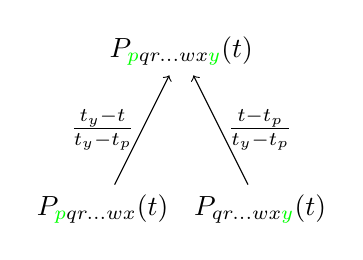
\begin{tikzpicture}
							\node (x) at (0, 0) {$P_{{\color{green}p}qr...wx}(t)$};
							\node (z) at (1, 2) {$P_{{\color{green}p}qr...wx{\color{green}y}}(t)$};
							\node (y)at (2, 0) {$P_{qr...wx{\color{green}y}}(t)$};
		
							\draw[->] (x) -- node[xshift=-0.5cm]{$\frac{t_y - t}{t_y - t_p}$} (z);
							\draw[->] (y) -- node[xshift=0.5cm]{$\frac{t - t_p}{t_y - t_p}$} (z);
						\end{tikzpicture}
					\end{figure}	
					\item Indien echter in de labeling van een hulppunt, of van het eindresultaat, slechts één enkele index $i$ optreedt, met multipliciteit $\mu_i = m + 1$, dan moet op het lager niveau slechts één enkel hulppunt geïntroduceerd worden: het hulppunt waarin de index $i$ optreedt met multipliciteit $\mu_i = m$.
					\begin{figure}[ht]
						\centering
						\begin{tikzpicture}
							\node (x) at (0, 0) {$P_{i}^{(m)}$};
							\node (z) at (1, 2) {$\substack{P_{\underline{i...i}}(t) \\ \hbox{\scriptsize {m+1 termen}}}$};
							\node (y)at (2, 0) {$\substack{P_{\underline{i...i}}(t) \\ \hbox{\scriptsize {m termen}}}$};
		
							\draw[->] (x) -- node[xshift=-0.5cm]{$\frac{(t - t_i)^m}{m!}$} (z);
							\draw[->] (y) -- node[xshift=0.5cm]{$1$} (z);
						\end{tikzpicture}
					\end{figure}	
						
				\end{enumerate}
				Veronderstel nu een Hermite interpolatie van graad vijf. Dit heeft twee datapunten $P_0$ en $P_1$, de richtingsvectoren in deze punten $P_0^{'}$ en $P_1^{'}$, en de krommingen $P_0^{''}$ en $P_{1}^{''}$. Punt $P_{000111}(t)$ is de top van het piramidaal schema. Op figuur \ref{fig:20triangular} wordt dit schema voorgesteld.

				\begin{figure}[ht]
					\centering
					\begin{tikzpicture}[scale=1.5]
						\node (p000111) at (5, 10) {$P_{000111}(t)$};
							\node (p00011) at (4, 8) {$P_{00011}(t)$};
							\node (p00111) at (6, 8) {$P_{00111}(t)$};
								\node (p0001) at (3, 6) {$P_{0001}(t)$};
								\node (p0011) at (5, 6) {$P_{0011}(t)$};
								\node (p0111) at (7, 6) {$P_{0111}(t)$};
									\node (p000) at (2, 4) {$P_{000}(t)$};
									\node (p001) at (4, 4) {$P_{001}(t)$};
									\node (p011) at (6, 4) {$P_{011}(t)$};
									\node (p111) at (8, 4) {$P_{111}(t)$};
										\node (p0'') at (1, 2) {$P_{0}^{''}$};
										\node (p00) at (3, 2) {$P_{00}(t)$};
										\node (p01) at (5, 2) {$P_{01}(t)$};
										\node (p11) at (7, 2) {$P_{11}(t)$};
										\node (p1'') at (9, 2) {$P_{1}^{''}$};
											\node (p0') at (2, 0) {$P_{0}^{'}$};
											\node (p0) at (4, 0) {$P_{0}$};
											\node (p1) at (6, 0) {$P_{1}$};
											\node (p1') at (8, 0) {$P_{1}^{'}$};
						
						\draw[->] (p0') -- node[xshift=-0.5cm]{t} (p00);
						\draw[->] (p0) -- node[xshift=0.2cm]{1} (p00);
						\draw[->] (p0) -- node[xshift=-0.5cm]{1 - t} (p01);
						\draw[->] (p1) -- node[xshift=0.2cm]{t} (p01);
						\draw[->] (p1) -- node[xshift=-0.2cm]{t}(p11);
						\draw[->] (p1') -- node[xshift=0.5cm]{t - 1} (p11);

						\draw[->] (p0'') -- node[xshift=-0.5cm]{$\frac{t^2}{2}$} (p000);
						\draw[->] (p00) -- node[xshift=0.2cm]{1} (p000);
						\draw[->] (p00) -- node[xshift=-0.5cm]{1 - t} (p001);
						\draw[->] (p01) -- node[xshift=0.2cm]{t}  (p001);

						\draw[->] (p01) -- node[xshift=-0.5cm]{1 - t}(p011);
						\draw[->] (p11) -- node[xshift=0.2cm]{t} (p011);
						\draw[->] (p11) -- node[xshift=-0.2cm]{1}(p111);
						\draw[->] (p1'') -- node[xshift=0.5cm]{$\frac{(t - 1)^2}{2}$}  (p111);

						\draw[->] (p000) -- node[xshift=-0.5cm]{1 - t}(p0001);
						\draw[->] (p001) -- node[xshift=0.2cm]{t}(p0001);
						\draw[->] (p001) -- node[xshift=-0.5cm]{1 - t} (p0011);
						\draw[->] (p011) -- node[xshift=0.2cm]{t}(p0011);
						\draw[->] (p011) -- node[xshift=-0.5cm]{1 - t} (p0111);
						\draw[->] (p111) -- node[xshift=0.2cm]{t} (p0111);

						\draw[->] (p0001) -- node[xshift=-0.5cm]{1 - t}(p00011);
						\draw[->] (p0011) -- node[xshift=0.2cm]{t}(p00011);
						\draw[->] (p0011) -- node[xshift=-0.5cm]{1 - t} (p00111);
						\draw[->] (p0111) -- node[xshift=0.2cm]{t}(p00111);

						\draw[->] (p00011) -- node[xshift=-0.5cm]{1 - t}(p000111);
						\draw[->] (p00111) -- node[xshift=0.2cm]{t}(p000111);				
					\end{tikzpicture}
					\caption{}
					\label{fig:20triangular}
				\end{figure}

		\end{itemize}}
		De gewichtsfuncties kunnen berekent worden via de volgende stappen:
		\begin{enumerate}
			\item Keer elke pijl van het schema om.
			\item Plaats de constante 1 op de top van de piramide.
			\item De mengfunctie horend bij een specifiek basisdatapunt $P_i$, kan bekomen worden door in het aangepaste diagram achtereenvolgens:
				\begin{enumerate}
					\item het aantal alternatieve paden te zoeken die tot dit punt leiden (eenvoudig via de driehoek van Pascal),
					\item de gewichtsfactoren langs een specifiek pad te vermenigvuldigen,
					\item de bijdrage van elk individueel pad te sommeren.
				\end{enumerate}
		\end{enumerate}

		Op figuur\ref{fig:20invtriangular} wordt het omgekeerde schema getoond.

		\begin{figure}[ht]
			\centering
			\begin{tikzpicture}[scale=1.5]
				\node (p000111) at (5, 10) {};
					\node (p00011) at (4, 8){};
					\node (p00111) at (6, 8) {};
						\node (p0001) at (3, 6) {};
						\node (p0011) at (5, 6) {};
						\node (p0111) at (7, 6) {};
							\node (p000) at (2, 4) {};
							\node (p001) at (4, 4) {};
							\node (p011) at (6, 4) {};
							\node (p111) at (8, 4) {};
								\node (p0'') at (1, 2) {$H_{2,5}(t)$};
								\node (p00) at (3, 2) {};
								\node (p01) at (5, 2) {};
								\node (p11) at (7, 2) {};
								\node (p1'') at (9, 2) {$H_{3,5}(t)$};
									\node (p0') at (2, 0) {$H_{1,5}(t)$};
									\node (p0) at (4, 0) {$H_{0,5}(t)$};
									\node (p1) at (6, 0) {$H_{5,5}(t)$};
									\node (p1') at (8, 0) {$H_{4,5}(t)$};
				
				\draw[<-] (p0') -- node[xshift=-0.5cm]{t} (p00);
				\draw[<-] (p0) -- node[xshift=0.2cm]{1} (p00);
				\draw[<-] (p0) -- node[xshift=-0.5cm]{1 - t} (p01);
				\draw[<-] (p1) -- node[xshift=0.2cm]{t} (p01);
				\draw[<-] (p1) -- node[xshift=-0.2cm]{t}(p11);
				\draw[<-] (p1') -- node[xshift=0.5cm]{t - 1} (p11);

				\draw[<-] (p0'') -- node[xshift=-0.5cm]{$\frac{t^2}{2}$} (p000);
				\draw[<-] (p00) -- node[xshift=0.2cm]{1} (p000);
				\draw[<-] (p00) -- node[xshift=-0.5cm]{1 - t} (p001);
				\draw[<-] (p01) -- node[xshift=0.2cm]{t}  (p001);

				\draw[<-] (p01) -- node[xshift=-0.5cm]{1 - t}(p011);
				\draw[<-] (p11) -- node[xshift=0.2cm]{t} (p011);
				\draw[<-] (p11) -- node[xshift=-0.2cm]{1}(p111);
				\draw[<-] (p1'') -- node[xshift=0.5cm]{$\frac{(t - 1)^2}{2}$}  (p111);

				\draw[<-] (p000) -- node[xshift=-0.5cm]{1 - t}(p0001);
				\draw[<-] (p001) -- node[xshift=0.2cm]{t}(p0001);
				\draw[<-] (p001) -- node[xshift=-0.5cm]{1 - t} (p0011);
				\draw[<-] (p011) -- node[xshift=0.2cm]{t}(p0011);
				\draw[<-] (p011) -- node[xshift=-0.5cm]{1 - t} (p0111);
				\draw[<-] (p111) -- node[xshift=0.2cm]{t} (p0111);

				\draw[<-] (p0001) -- node[xshift=-0.5cm]{1 - t}(p00011);
				\draw[<-] (p0011) -- node[xshift=0.2cm]{t}(p00011);
				\draw[<-] (p0011) -- node[xshift=-0.5cm]{1 - t} (p00111);
				\draw[<-] (p0111) -- node[xshift=0.2cm]{t}(p00111);

				\draw[<-] (p00011) -- node[xshift=-0.5cm]{1 - t}(p000111);
				\draw[<-] (p00111) -- node[xshift=0.2cm]{t}(p000111);				
			\end{tikzpicture}
			\caption{s}
			\label{fig:20invtriangular}
		\end{figure}
		
		De mengfuncties worden dan:
		\begin{equation*}
			\begin{split}
				H_{0, 5}(t) = & 6 \cdot \bigg[(1-t)^3 + t(1-t)^3 + 4t^2(1-t)^3\bigg] = -24t^5 + 66t^4 -60t^3 + 24t^2 -12t + 6\\
				H_{1, 5}(t) = & 4 \cdot \bigg[t(1-t)^3 + 3t^2(1-t)^3\bigg] = -12t^5 +32t^4 -24t^3 + 4t\\
				H_{2, 5}(t) = & 1 \cdot \bigg[(1 - t)^3\bigg(\frac{t^2}{2}\bigg)\bigg] = -\frac{1}{2}  t^5 + \frac{3}{2}  t^4  - \frac{3}{2}t^3 + \frac{1}{2}t^2\\
				H_{3, 5}(t) = & 1 \cdot \bigg[(t^3\bigg(\frac{(1-t)^2}{2}\bigg)\bigg] = \frac{1}{2}t^5 - t^4 + \frac{1}{2}t^3\\
				H_{4, 5}(t) = & 4 \cdot \bigg[a_4t^5 + b_4t^4 + c_4t^3 + d_4t^2 + e_4t + f_4 \bigg]  \\
				H_{5, 5}(t) = & 6 \cdot \bigg[a_5t^5 + b_5t^4 + c_5t^3 + d_5t^2 + e_5t + f_5 \bigg]  \\
			\end{split}
		\end{equation*}
		Omgevormd tot de matrixrepresentatie:
		$$
		P(t) = (t^5, t^4, t^3, t^2, t, 1) 
		\cdot
		\begin{pmatrix}
			-24 & -12 & - \frac{1}{2}  & \frac{1}{2} & a_4 & a_5 \\
			66  & 32  & \frac{3}{2}    & -1 		 & b_4 & b_5 \\
			-60 & -24 & - \frac{3}{2}  & \frac{1}{2} & c_4 & c_5 \\
			24  & 4   &  \frac{1}{2}   & 0 			 & d_4 & d_5 \\
			-12 & 0   & 0  			   & 0 			 & e_4 & e_5 \\
			6   & 0   & 0  			   & 0 			 & f_4 & f_5 \\
		\end{pmatrix}
		\cdot 
		\begin{pmatrix}
			P_0 \\
			P_1 \\
			P_0^{'} \\
			P_1^{''} \\
			P_0^{'} \\
			P_1^{''} \\

		\end{pmatrix}
		$$
		\accentuate{CONTROLE: Som van de waarden van de rijen voor elk datapunt moet 0 zijn: $-24 -12 - \frac{1}{2} + \frac{1}{2} + a_4 + a_5 = 0 $}.



			
\end{itemize}
\end{document}


